\documentclass[12pt,a4paper]{ctexart}
\usepackage[margin=2.5cm]{geometry}
\usepackage{graphicx}
\usepackage{pdfpages}
\usepackage{booktabs}
\usepackage{longtable}
\usepackage{array}
\usepackage{tabularx}
\usepackage{xltabular}
\usepackage{colortbl}
% 配合 xltabular 的可变列：L = 左对齐自适应列（自动填满版心），P{宽} = 居中定宽列
\newcolumntype{L}{>{\raggedright\arraybackslash}X}
\newcolumntype{P}[1]{>{\centering\arraybackslash}p{#1}}
% 左对齐定宽列：避免中文在窄列中被两端对齐拉伸、造成字距忽大忽小
\newcolumntype{Q}[1]{>{\raggedright\arraybackslash}p{#1}}
\usepackage{enumitem}
\usepackage{caption}
\usepackage{subcaption}
\usepackage{float}
\PassOptionsToPackage{hyphens}{url}
\usepackage{hyperref}
\usepackage{tikz}
\usetikzlibrary{positioning,calc,arrows.meta,shapes.geometric}
\usepackage{amsmath,amssymb}

% 统一箭头样式（活动图 / 时序图）
\tikzset{ >=Stealth }

\setlist{itemsep=2pt,parsep=0pt,topsep=4pt}
% 一级列表（enumerate）：左缩进设为 0，编号顶格，条目文字紧随其后
\setlist[enumerate]{labelindent=0.8em, itemindent=0pt, labelsep=0.5em, leftmargin=*}
% 嵌套在有序列表内的紧凑无序列表（subbullet）：收紧左缩进与条目间距，避免层级缩进过长
\newlist{subbullet}{itemize}{1}
\setlist[subbullet]{label=\textbullet, leftmargin=1em, labelindent=0.2em, itemindent=0pt, labelsep=0.3em, topsep=2pt, itemsep=1pt, parsep=0pt}
% 表格单元格内的紧凑无序列表：当单元格含多条内容时，用项目符号逐条罗列，且不留额外空隙
\newlist{celllist}{itemize}{1}
% 说明：列表作为 p 列单元格的首个内容时，其基准点落在列表顶部而非首行基线，
% 使首行比同行单行单元格（基准点=文本基线）低约一个汉字字高（12pt 下约 9.8pt）。
% 用负的 before 间距把整列上提，使右侧首行与左侧标题首行齐平。
\setlist[celllist]{label=\textbullet, leftmargin=*, labelsep=0.5em, topsep=0pt, partopsep=0pt, itemsep=0pt, parsep=0pt, before={\vspace{-9.8pt}}}
% 表格单元格内的紧凑编号列表：用于逐条罗列验收检查点，编号为 1. 2. 3.
\newlist{cellenum}{enumerate}{1}
\setlist[cellenum]{label=\arabic*., leftmargin=*, labelsep=0.5em, topsep=0pt, partopsep=0pt, itemsep=2pt, parsep=0pt, before={\vspace{-9.8pt}}}
\captionsetup{font=small,labelfont=bf,skip=6pt,aboveskip=3pt}
\hypersetup{colorlinks=true,linkcolor=black,urlcolor=blue}
% 表格整体排版：适当加宽行距与单元格左右内边距
\renewcommand{\arraystretch}{1.4}
\setlength{\tabcolsep}{7pt}
% 收紧长表格（xltabular/longtable）与前后文的纵向间距：默认 \bigskipamount（12pt）偏大，
% 会让表格在页尾“整块跳页”并在标题后留出较大空隙；降到 4pt 使表格更贴近上下文、更易跨页续排
\setlength{\LTpre}{4pt}
\setlength{\LTpost}{4pt}
\emergencystretch=2em
% 表内行间浅分割线（比 \midrule 更细、颜色更浅，用于区分各行）
\newcommand{\rowrule}{\arrayrulecolor[gray]{0.7}\specialrule{0.3pt}{0.4ex}{0.4ex}\arrayrulecolor[gray]{0}}
% 标题与上下文的间距：收紧 section（一级）/ subsection（二级）标题的上下留白
\ctexset{
  section = {
    beforeskip = 2ex plus 0.5ex minus 0.2ex,
    afterskip  = 1ex plus 0.2ex minus 0.1ex,
  },
  subsection = {
    beforeskip = 1.5ex plus 0.4ex minus 0.2ex,
    afterskip  = 1ex plus 0.2ex minus 0.1ex,
  },
}

\begin{document}

\begin{titlepage}
\centering
\vspace*{1.5cm}

\includegraphics[width=6cm]{images/logo.jpg}\par
\vspace{1.2cm}
{\Huge\bfseries
《膳食搭配智能体系统》\par
\vspace{1em}
 软件需求规格说明书}
\vspace{2cm}


\begin{tabular}{cc}
\textbf{团队名称} & 海底小纵队 \\
\textbf{文档版本} & v2.0 \\
\textbf{编制日期} & 2026-11-14 \\
\textbf{编制人} & 李铭媛（PM）、李思淇、洪雅琳 \\
\end{tabular}
\vfill
{\large 依从 GB/T 9385---2008\par}
\end{titlepage}

% 前置部分（迭代记录表、目录）采用罗马数字页码，正文从第一章起改用阿拉伯数字
\pagenumbering{roman}

\begin{xltabular}{\linewidth}{P{1cm}P{1cm}p{1.7cm}LP{2cm}}
\caption{迭代记录表} \\
\toprule
\textbf{版本} & \textbf{日期} & \textbf{修改人} & \textbf{修改内容} \\
\midrule
\endhead
v0.1 & 10/16 & 李铭媛 & 建立文档骨架，列出各章节   \\
v0.2 & 10/17 & 李铭媛 & 排版封面与 Logo，撰写第一章、2.4-2.6 节   \\
v0.3 & 10/17 & 李思淇 & 撰写 2.3 节、3.2 节、附录 A  \\
v0.4 & 10/17 & 洪雅琳 & 撰写 2.1-2.2、3.1.2、3.3-3.5、第四章、第五章、附录 B  \\
v1.0 & 10/18 & 李铭媛 & 整合排版，统一文风，组织整体书写逻辑   \\
v1.1 & 10/19 & 李思淇 & 更新 3.1.1 用户界面介绍  \\
v1.2 & 10/19 & 洪雅琳 & 更新思维导图  \\
v1.3 & 10/20 & 李铭媛 & 补充时序图、活动图；更新 1.4 引用文件；优化排版布局   \\
v1.4 & 10/21 & 李铭媛 & 全文校对定稿   \\
v2.0 & 11/14 & 李铭媛 & 按产品方案 v1.2 对齐全文口径，并更新类图 / 时序图 / 原型图 \\
\bottomrule
\end{xltabular}

% ============ 目录 ============
\newpage
\tableofcontents
\newpage

% 正文页码从第一章开始（阿拉伯数字，重新从 1 计数）
\pagenumbering{arabic}

\section{引言}

\subsection{目的}

本文档定义「膳食搭配智能体系统」的软件需求，说明系统的目标用户、使用场景、功能与非功能需求，以及领域智能体的定制方法与验收标准。
本文档的预期读者包括：

\begin{itemize}
\item 项目开发团队（前端、后端、Agent定制、数据岗），作为设计与开发的依据；
\item 测试与交付人员，作为测试用例与验收的依据；
\item 课程老师与助教，用于评审选题与项目范围。
\end{itemize}

\subsection{范围}

本SRS适用于“膳食搭配智能体系统”软件产品，该系统面向有意识调控饮食、以自行烹饪为主的用户，采用“营养搭配 $\rightarrow$ 菜式落地”两步模型，提供个性化膳食配餐服务。
系统的主要功能概要见~\ref{sec:product-function}；各功能的实现阶段与优先级（基本 / 有条件 / 可选）以及推迟至后续版本实现的功能，见~\ref{sec:req-allocation} 需求分配。

本系统应用于个人日常膳食管理场景，旨在帮助不具备系统营养学知识的用户获得可执行、可解释、可计算的家常菜配餐方案，降低膳食管理门槛，提升饮食控制的可行性与持续性，支持合理膳食、体重管理及营养相关慢性病风险因素的日常干预，使用户在长期均衡饮食中获得更充沛的精力与更健康的身体状态，提升日常生活质量。

\subsection{定义、简写和缩略语}

\begin{xltabular}{\linewidth}{p{3.5cm}L}
\caption{术语、简写和缩略语} \\
\toprule
\textbf{术语} & \textbf{定义} \\
\midrule
\endfirsthead
\toprule
\textbf{术语} & \textbf{定义} \\
\midrule
\endhead
智能体（Agent） & 调用大模型并编排工具完成领域任务的软件模块 \\
LLM & 大语言模型，选用 DeepSeek（经 Agno 框架接入） \\
RAG & 检索增强生成，从领域知识库检索资料辅助大模型回答 \\
Function Calling & 工具调用，智能体调用外部函数完成确定性计算 \\
JSON Schema & 约束智能体输出格式的 JSON 结构定义 \\
BMR & 基础代谢率，依据 Mifflin-St Jeor 公式计算 \\
固定活动系数 & 能量目标 = BMR $\times$ 1.4，仅作份量量级参考，不做热量缺口 / 盈余 \\
宏量营养素 & 碳水化合物、蛋白质、脂肪，按供能比例每餐配比 \\
微量营养素 & 维生素、矿物质，固定 7 种关键微量（钙、铁、锌、维 A、B1、B2、C）跨日动态平衡评估 \\
DRIs & 膳食营养素参考摄入量（Dietary Reference Intakes），含 RNI、AI（适宜摄入量）、UL（可耐受最高摄入量）等的推荐体系，本系统主要采用 RNI \\
RNI & 推荐摄入量（Recommended Nutrient Intake），满足绝大多数个体每日需要的营养素摄入水平，本系统用于微量营养素达标评估 \\
GI & 升糖指数，衡量食物升高血糖的速度 \\
生重口径 / \newline 成品口径 & 营养估算的两种口径：食材按未烹饪生重（每 100g）计、菜式按烹饪后成品（含做法与份量）计 \\
反向营养 & 由症状描述经多轮对话推测“可能缺乏的营养素”的能力 \\
意图路由 & 智能体将用户输入归入「询问 / 配餐 / 调整」三条处理路径之一 \\
方案状态机 & 方案状态 \texttt{draft}（生成中）$\rightarrow$ \texttt{candidates}（候选可换）$\rightarrow$ \texttt{fixed}（已固定只读锁定） \\
data\_quality 三态 & 数据质量三态 \texttt{official}（官方实测）/ \texttt{approx}（估算）/ \texttt{check}（待核查），仅 official 可作官方结论 \\
\bottomrule
\end{xltabular}

\subsection{引用文件}

\begin{enumerate}
\item 中华人民共和国国家质量监督检验检疫总局，中国国家标准化管理委员会. GB/T 9385---2008 计算机软件需求规格说明规范[S]. 2008-09-01 实施. 来源：国家标准全文公开系统。
\item 中华人民共和国国家标准. GB/T 11457---2006 信息技术 软件工程术语[S]. 来源：国家标准全文公开系统。
\item 中国营养学会. 中国居民膳食指南（2022）[M]. 北京：人民卫生出版社，2022. 来源：公开出版物。
\item 中国营养学会. 中国居民膳食营养素参考摄入量（2023版）[M]. 来源：中国营养学会官网。
\item 中国疾病预防控制中心营养与健康所. 中国食物成分表（标准版）[M]. 北京：北京大学医学出版社，2018. 来源：公开出版物；补充食材数据参考 USDA FoodData Central（FDC）。
\end{enumerate}

\subsection{综述}

本文档共分五章及附录：第 2 章总体描述介绍产品背景，包括产品描述、产品功能、用户特点、约束、假设与依赖关系、需求分配；第 3 章具体需求按系统特征组织，逐条描述功能、外部接口、性能、设计约束与软件系统属性；第 4 章给出数据/对象模型（类图）；第 5 章给出验收标准；附录提供调研结果与领域知识来源清单。

系统整体功能与结构的全景见图~\ref{fig:overview}。

\begin{figure}[H]
  \centering
  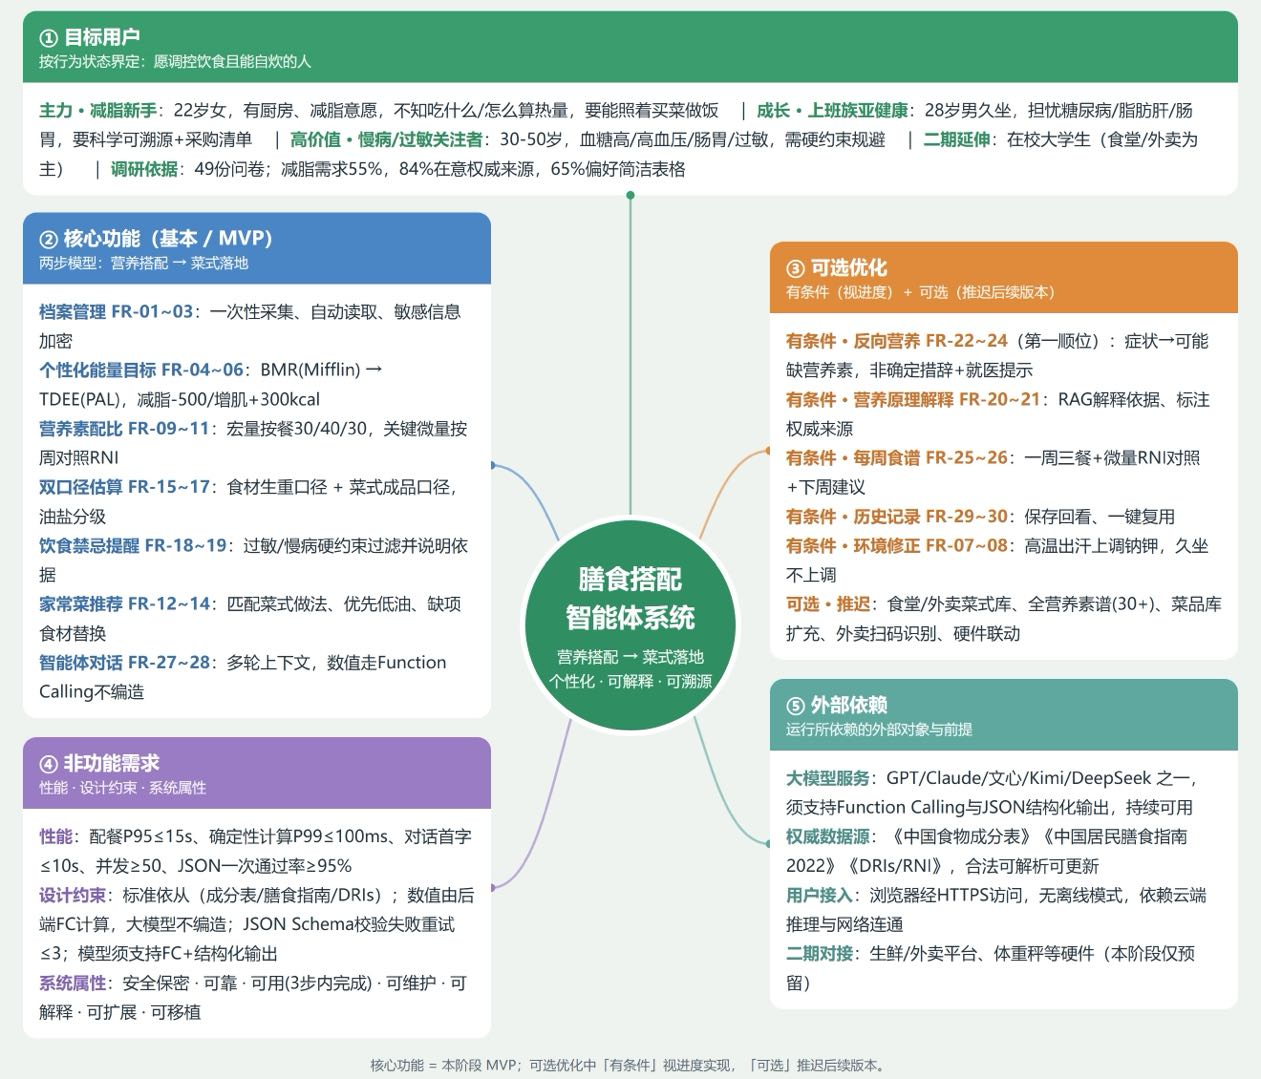
\includegraphics[width=0.55\textwidth]{images/overview.jpg}
  \caption{系统全景图}
  \label{fig:overview}
\end{figure}

\section{总体描述}

\subsection{产品描述}

本产品「膳食搭配智能体系统」是一款面向\textbf{有意识调控饮食、以自行烹饪为主}人群的纯软件 Web 应用，以「营养素配比平衡」为核心，采用「营养搭配 $\rightarrow$ 菜式落地」两步模型，将个性化营养方案（食材层）落地为可执行的家常菜菜单（菜式层），并全程标注依据来源。

本产品是一个\textbf{独立、自我包含}的软件系统，不隶属于其他更大系统；其运行\textbf{依赖的外部对象仅大模型服务}，提供自然语言理解、函数调用（Function Calling）与结构化输出能力。权威数据源（《中国食物成分表》《中国居民膳食指南（2022）》及 RNI 标准）经数据侧清洗与口径统一后\textbf{离线入库}至系统内部数据库（PostgreSQL + pgvector），供知识检索与确定性计算使用，运行时不再依赖外部数据源。产品与外部实体之间的接口关系如下图所示：

\begin{figure}[H]
  \centering
  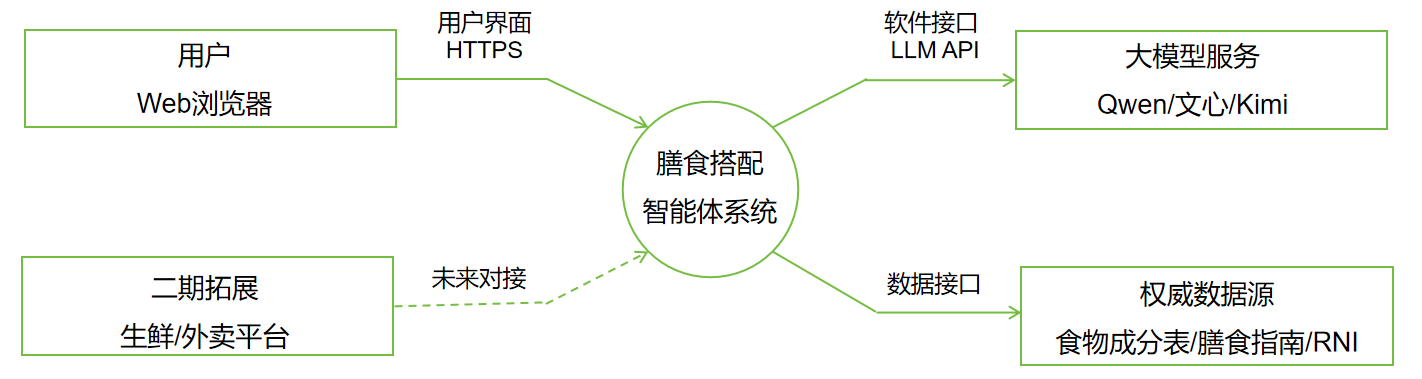
\includegraphics[width=\textwidth]{images/接口关系示意图.png}
  \caption{产品与外部实体之间的接口关系示意图}
  \label{fig:reliance_demo}
\end{figure}

「营养搭配 $\rightarrow$ 菜式落地」两步业务流程见图~\ref{fig:activity_flow}：第一步在食材层完成能量目标与营养素配比，并针对饮食禁忌做硬约束过滤；第二步在菜式层落地为家常菜并估算热量与营养素，最终输出可溯源的配餐方案。

\begin{figure}[H]
  \centering
  \resizebox{!}{0.58\textheight}{%
  \begin{tikzpicture}[
    font=\small,
    act/.style={draw,rounded corners=3pt,align=center,minimum width=4.3cm,minimum height=0.85cm,inner sep=3pt},
    dec/.style={draw,diamond,aspect=2.2,align=center,minimum width=3.4cm,minimum height=1.9cm,inner sep=0pt,font=\small},
    start/.style={draw,circle,fill,minimum size=0.4cm,inner sep=0pt},
    end/.style={draw,circle,double,double distance=1.5pt,minimum size=0.6cm,inner sep=0pt},
    merge/.style={draw,circle,fill,minimum size=0.25cm,inner sep=0pt},
  ]
    % 第一步：营养搭配（食材层）
    \draw[dashed,rounded corners,color=black!55] (-3.3,8.8) rectangle (7.1,1.2);
    \node[anchor=north west,font=\scriptsize\bfseries,color=black!70] at (-3.2,8.75) {第一步：营养搭配};
    \node[anchor=north east,font=\scriptsize\bfseries,color=black!70] at (7.0,8.75) {食材层};
    % 第二步：菜式落地（菜式层）
    \draw[dashed,rounded corners,color=black!55] (-3.3,0.3) rectangle (7.1,-5.6);
    \node[anchor=north west,font=\scriptsize\bfseries,color=black!70] at (-3.2,0.25) {第二步：菜式落地};
    \node[anchor=north east,font=\scriptsize\bfseries,color=black!70] at (7.0,0.25) {菜式层};

    \node[start] (st) at (0,9.4) {};
    \node[act] (a1) at (0,7.6) {读取 / 填写个人健康档案};
    \node[act] (a2) at (0,5.8) {计算个性化能量目标\\（BMR × 1.4，份量量级）};
    \node[act] (a3) at (0,4.0) {营养素配比\\（宏量按餐、微量跨日平衡）};
    \node[dec] (d1) at (0,2.0) {存在禁忌\\或过敏？};
    \node[act] (a4) at (4.9,2.0) {饮食禁忌\\硬约束过滤};
    \node[merge] (m1) at (0,-0.1) {};
    \node[act] (a5) at (0,-1.2) {家常菜推荐\\（菜式落地 + 烹饪方式 / 油盐估算）};
    \node[act] (a6) at (0,-3.0) {热量与营养素估算\\（食材 / 菜式双口径）};
    \node[act] (a7) at (0,-4.8) {标注权威依据来源};
    \node[act] (a8) at (0,-6.8) {输出配餐方案};
    \node[end] (en) at (0,-8.6) {};

    \draw[->] (st) -- (a1);
    \draw[->] (a1) -- (a2);
    \draw[->] (a2) -- (a3);
    \draw[->] (a3) -- (d1);
    \draw[->] (d1) -- node[above,font=\scriptsize]{是} (a4);
    \draw[->] (a4) |- (m1);
    \draw[->] (d1) -- node[left,font=\scriptsize]{否} (m1);
    \draw[->] (m1) -- (a5);
    \draw[->] (a5) -- (a6);
    \draw[->] (a6) -- (a7);
    \draw[->] (a7) -- (a8);
    \draw[->] (a8) -- (en);
  \end{tikzpicture}}
  \caption{配餐业务流程活动图（营养搭配 $\rightarrow$ 菜式落地）}
  \label{fig:activity_flow}
\end{figure}

外部接口的高层识别如下（各接口的详细定义见~\ref{sec:interfaces}）：

\begin{xltabular}{\linewidth}{p{2.2cm}LP{2.0cm}}
\caption{外部接口高层识别} \\
\toprule
\textbf{接口类型} & \textbf{说明} & \textbf{详细定义} \\
\midrule
\endfirsthead
\toprule
\textbf{接口类型} & \textbf{说明} & \textbf{详细定义} \\
\midrule
\endhead
用户界面 & 浏览器访问的 Web 前端，以对话交互为主 & 3.1.1 \\
软件接口 & 大模型 API，须支持函数调用与结构化（JSON）输出 & 3.1.2 \\
数据接口 & 内部数据库（PostgreSQL + pgvector）：关系表存数值基准、向量存文本知识，权威数据源离线入库 & 3.1.2 \\
硬件接口 & 无（纯软件项目，不涉及硬件联动） & --- \\
通信接口 & HTTPS & --- \\
\bottomrule
\end{xltabular}

就「置于相关产品全景」而言，本产品是\textbf{通用大模型的领域定制}：通过领域知识、规则计算与工具编排，补齐其无法精确计算能量与营养素、微量不配比、无权威溯源的短板；相较通用营养类 App，本产品以「营养素配比平衡」为核心并全程可溯源，而非仅做热量记录；未来可进一步对接体重秤、生鲜与外卖平台（见~\ref{sec:req-allocation} 二期需求）。

系统以\textbf{交互式对话}为主要运行方式：用户经浏览器发起配餐或咨询请求，系统在线调用大模型与数据源完成计算与推荐，无离线模式。

\textbf{内存约束}：系统为轻量 Web 应用，服务端无专用算力，大模型推理走云端 API，内存与硬件资源要求低（详见~\ref{sec:constraints}）。

\textbf{现场适应性}：运行于通用浏览器与标准服务器环境，无特殊现场安装要求。

\subsection{产品功能}\label{sec:product-function}

主要功能按模块概述如下：

\begin{enumerate}
\item \textbf{人机交互与档案管理}
  \begin{subbullet}
  \item 对话交互入口：用户以自然语言发起配餐、营养查询等请求。
  \item 用户档案管理：维护身体信息、健康信息（疾病/过敏/禁忌）、饮食偏好与健康目标。
  \item 历史方案：保存历史配餐方案，供回看与复用。
  \end{subbullet}
\item \textbf{智能生成个性化营养膳食方案}
  \begin{subbullet}
  \item 个性化能量与营养目标计算：依据档案计算 BMR $\times$ 1.4 能量目标（份量量级，不做热量缺口），健康目标只改结构。
  \item 营养素配比：宏量营养素按每餐配比，7 种关键微量跨日动态平衡。
  \item 热量与营养素估算：食材按生重口径、菜式按成品口径分别核算。
  \item 饮食禁忌提醒：依据疾病、过敏与禁忌信息做硬约束过滤。
  \item 家常菜推荐：从家常菜库匹配菜式，给出烹饪方式与油盐估算。
  \item 候选生成与调整：每餐 2~3 个候选，支持「换一换」与「确认/固定」。
  \item 膳食报告：汇总已确认方案，输出周/月营养复盘与调整建议。
  \end{subbullet}
\item \textbf{咨询与原理解释}
  \begin{subbullet}
  \item 反向营养咨询：由症状描述推测可能缺乏的营养素并给出食物建议。
  \item 营养原理解释：解释配餐背后的营养学依据。
  \end{subbullet}
\end{enumerate}

各功能的实现阶段与优先级（基本 / 有条件 / 可选）以及本阶段不实现的功能，详见~\ref{sec:req-allocation} 需求分配。

\subsection{用户特点}

\subsubsection{调研依据与数据来源}

\begin{enumerate}
  \item \textbf{调研方式}：采用在线问卷的形式，共收集了49份有效样本，题目覆盖基础信息、饮食现状与痛点、功能需求、使用偏好、开放建议。
  \item \textbf{样本构成}：18--25 岁占 81.63\%；女性 61.22\%、男性 38.78\%；BMI 正常 75.51\%；55.10\% 存在减脂/体重管理需求；53.06\% 至少担忧一项慢性问题（糖尿病 32.65\%、胃肠道 22.45\%、心脑血管 22.45\%）；24.49\% 现患至少一项慢性情况；18.37\% 存在食物过敏。
  \item \textbf{调研局限说明}：样本以 18--25 岁在校学生为主，该群体以食堂/外卖就餐为主，与本阶段“自行烹饪”的产品定位存在偏差。因此本阶段目标用户不按人口身份、而按“是否具备自炊条件”界定（见~\ref{sec:user-general}）；在校学生群体列为二期延伸对象（见~\ref{sec:user-persona}）。
  \item \textbf{调研发现}：（具体数据见\hyperref[appendix:a]{附录 A}）
  \begin{subbullet}
    \item \textbf{就餐方式}：至少一半时间自行做饭 38.77\%（自炊为主 26.53\%）；外卖为主 61.22\%。
    \item \textbf{核心痛点}：“知道要吃健康但不知吃什么” 53.06\%；“不会算热量” 48.98\%；“买菜做饭麻烦” 24.49\%。
    \item \textbf{知识来源}：短视频 71.43\%、社交平台 57.14\%，专业渠道仅 10.20\%；用过同类工具者仅 36.73\%。
    \item \textbf{权威性}：83.67\% 在意方案是否参考权威资料。
    \item \textbf{功能优先级}：“非常需要”最高为饮食禁忌提醒 53.06\%；最看重 3 项为个性化方案+档案 75.51\%、自动算热量 57.14\%、禁忌提醒 40.82\%。
    \item \textbf{输出形式}：偏好简洁表格 65.31\%，“纯文字”为 0\%。
    \item \textbf{外卖/生鲜对接}：95.92\% 认可价值（很希望 57.14\% + 非必需 38.78\%），仅 4.08\% 不需要。
  \end{subbullet}
\end{enumerate}

调研主要发现的可视化统计见图~\ref{fig:survey_result}。

\begin{figure}[hbt]
  \centering
  \begin{subfigure}[b]{0.48\linewidth}
    \centering
    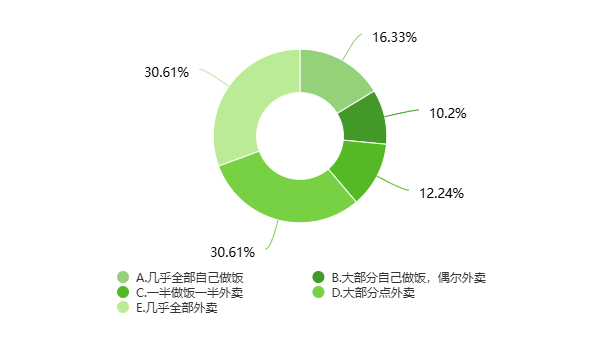
\includegraphics[width=\linewidth]{images/调查者用餐形式统计.png}
    \caption{用餐形式统计}
  \end{subfigure}\hfill
  \begin{subfigure}[b]{0.48\linewidth}
    \centering
    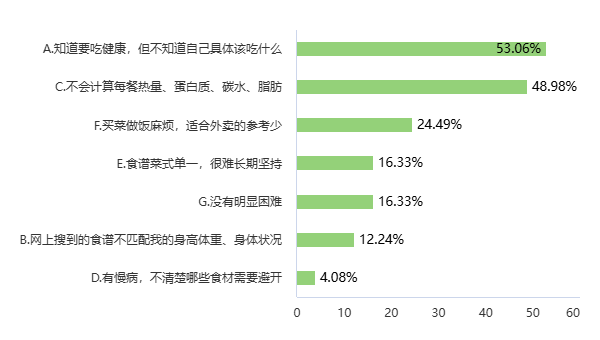
\includegraphics[width=\linewidth]{images/调查者在膳食方面的困难.png}
    \caption{膳食方面的困难}
  \end{subfigure}

  \vspace{1em}

  \begin{subfigure}[b]{0.48\linewidth}
    \centering
    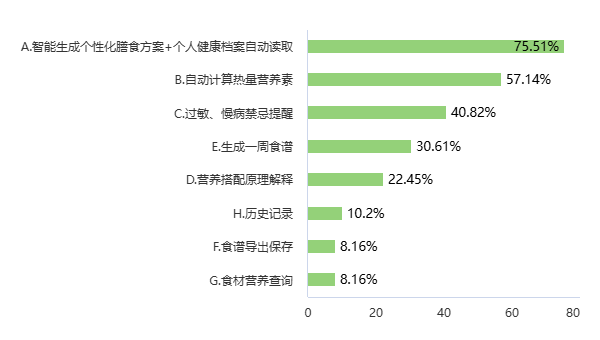
\includegraphics[width=\linewidth]{images/调查者最看重的功能.png}
    \caption{最看重的功能}
  \end{subfigure}\hfill
  \begin{subfigure}[b]{0.48\linewidth}
    \centering
    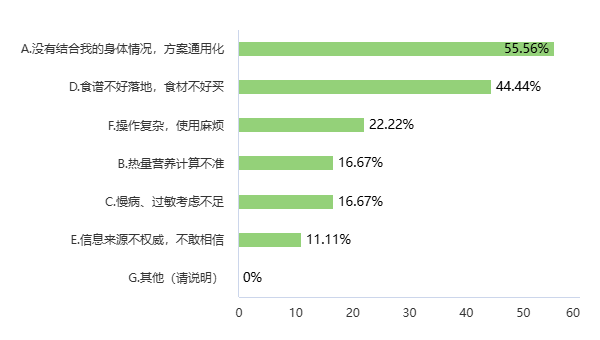
\includegraphics[width=\linewidth]{images/调查者认为现有APP存在的不足.png}
    \caption{现有同类 APP 存在的不足}
  \end{subfigure}

  \caption{用户调研结果统计}
  \label{fig:survey_result}
\end{figure}

\subsubsection{预期用户的一般特征}\label{sec:user-general}

本系统的价值目标不是替用户点餐，而是\textbf{帮助用户形成“有意识调控饮食、自行准备餐食”的自主能力}。据此，目标用户按行为状态而非人口属性界定：有意愿调控饮食、且愿意或已开始自行准备餐食的人。

\begin{enumerate}
\item \textbf{教育程度}。以高中及以上学历、大专/本科为主（以 18--25 岁青年为主），具备基本健康意识与信息检索能力，但不具备营养学专业知识，难以理解营养素配比、RNI 推荐摄入量等概念。
\item \textbf{使用经验}。为数字产品高频使用者，但专业饮食管理工具经验薄弱：仅少数用过饮食类 APP 或 AI 生成食谱，多数完全没接触；知识主要来自短视频与社交平台，碎片化、非权威；已有一定对话式 AI 使用习惯。
\item \textbf{专业技术情况}。 为消费级普通用户，非营养/医学专业人员，能熟练对话式交互，但普遍不会自行计算热量与营养素、缺乏慢病与食材对应知识。因此系统须以自然语言对话与结构化表格替代专业计算过程，做到“开箱即用”。
\item \textbf{目标用户边界与价值延伸路径}。一期聚焦“愿意调控饮食、且能够自行准备餐食”的用户------调研中“至少一半时间自行做饭”者占相当比例，是本期产品闭环可直接服务的对象。以食堂/外卖为主的用户需求同样真实（多数认可对接外卖/生鲜价值），但其中相当比例明确表示“非必需”，说明“一期先聚焦自炊、二期再接入外卖”是用户可接受的阶段性安排。延伸路径：一期在“自行准备”场景形成从“知道该吃什么”到“亲手做出一餐”的完整闭环；二期接入食堂/外卖常见菜式库，作为同一价值目标在“不做饭的日子”的延伸------先让用户会自己吃对，再让用户在外吃也对。
\end{enumerate}

\subsubsection{目标用户画像卡}\label{sec:user-persona}

\noindent \textbf{(1) 有自炊条件的年轻用户 $\cdot$ 减脂新手（本期主力画像）}

\begin{xltabular}{\linewidth}{p{2.0cm}L}
\caption{目标用户画像卡（一）：有自炊条件的减脂新手} \\
\toprule
\textbf{维度} & \textbf{描述} \\
\midrule
\endfirsthead
\toprule
\textbf{维度} & \textbf{描述} \\
\midrule
\endhead
基本信息 & 女，22 岁，有减脂/健康管理意愿，合租或独居有厨房、具备自炊条件，暂无慢病 \\
背景数据 & 减脂需求旺盛；具备自炊条件 \\
目标 & 想减脂、吃得健康，但不知道“具体该吃什么、吃多少、怎么做” \\
痛点 & 知道要吃健康却不知具体吃法；不会算热量；食谱难落地 \\
典型原话 & “在规定食材的情况下生成食谱”；“想要菜谱” \\
核心诉求 & 个性化、可落地、能照着买菜做饭；操作简单 \\
\bottomrule
\end{xltabular}

\noindent \textbf{(2) 年轻上班族 $\cdot$ 亚健康担忧者（本期成长画像）}

\begin{xltabular}{\linewidth}{p{2.0cm}L}
\caption{目标用户画像卡（二）：年轻上班族·亚健康担忧者} \\
\toprule
\textbf{维度} & \textbf{描述} \\
\midrule
\endfirsthead
\toprule
\textbf{维度} & \textbf{描述} \\
\midrule
\endhead
基本信息 & 男，28 岁，久坐办公，有厨房但缺乏时间规划，担忧糖尿病/脂肪肝/肠胃问题 \\
背景数据 & 担忧慢病风险；非常在意权威来源 \\
目标 & 控制体重与慢病风险，希望方案“科学、有依据、能快速执行” \\
痛点 & 方案通用化、不结合身体情况；食谱不好落地、食材不好买；热量计算不准 \\
典型原话 & “增加食材一键替换$\ldots$自动推荐同营养替代方案；支持按日/周生成采购清单”；“热量计算准确一点，配餐科学一点” \\
核心诉求 & 按身体条件个性化计算、结论可溯源、附采购清单便于执行 \\
\bottomrule
\end{xltabular}

\noindent \textbf{(3) 慢病 / 过敏关注者（本期高价值细分画像）}

\begin{xltabular}{\linewidth}{p{2.0cm}L}
\caption{目标用户画像卡（三）：慢病 / 过敏关注者} \\
\toprule
\textbf{维度} & \textbf{描述} \\
\midrule
\endfirsthead
\toprule
\textbf{维度} & \textbf{描述} \\
\midrule
\endhead
基本信息 & 30--50 岁，存在血糖偏高/高血压/胃肠道问题或食物过敏，具备自炊条件 \\
背景数据 & 存在过敏或禁忌；“饮食禁忌提醒”非常需要（全项最高） \\
目标 & 避免误食禁忌食材，安全地管理日常饮食 \\
痛点 & 有慢病不清楚需避开的食材；现有工具对慢病、过敏考虑不足 \\
典型原话 & “主要是健康方面”；“能更细化的表达和描述” \\
核心诉求 & 过敏/慢病硬约束规避与提醒、措辞安全、必要时提示就医 \\
\bottomrule
\end{xltabular}

\noindent \textbf{二期延伸画像}（本阶段暂不服务）：在校大学生 $\cdot$ 食堂/外卖为主。
该群体是调研样本主体（以 18--25 岁为主），减脂需求同样旺盛，但受食堂/外卖就餐场景所限，一期仅能帮助其先建立“知道该吃什么”的调控意识；待二期接入食堂/外卖常见菜式库后再完整服务其落地需求。

\subsubsection{典型使用场景}
\begin{enumerate}
  \item \textbf{对话配餐$\cdot$自炊落地}: 有减脂需求的年轻用户晚上打开系统，输入“帮我配明天的减脂餐”，系统依据其档案中的身高体重与减脂目标算出能量与营养目标，给出三餐搭配、做法与油盐估算，用户照着买菜做饭。
  \item \textbf{热量营养素估算}: 用户录入“中午吃了 150g 鸡胸肉、半碗米饭、一盘炒青菜”，系统自动给出这一餐的总热量及蛋白质、碳水、脂肪克数，帮助判断是否超标。
  \item \textbf{慢病 / 过敏安全配餐}: 有糖尿病且对花生过敏的用户配餐时，系统自动避开高 GI 食材和花生，并说明规避原因，让用户吃得放心。
  \item \textbf{档案复用}: 用户首次填写身高体重、慢病、过敏、口味偏好后，之后每次对话系统自动读取档案生成方案，无需重复描述自身情况。
\end{enumerate}

\textbf{二期扩展方向（本阶段不实现）}：详见~\ref{sec:req-allocation} 需求分配。

\subsubsection{用户特点对第 3 章需求的约束说明}
\vspace{-0.5em}
\begin{xltabular}{\linewidth}{p{6cm}Lp{4cm}}
\caption{用户特点对第 3 章需求的约束说明} \\
\toprule
\multicolumn{1}{c}{\textbf{用户特征/调研发现}} & \multicolumn{1}{>{\centering\arraybackslash}X}{\textbf{第 3 章对应条款}} & \multicolumn{1}{c}{\textbf{规定理由}} \\
\midrule
\endfirsthead
\toprule
\multicolumn{1}{c}{\textbf{用户特征/调研发现}} & \multicolumn{1}{>{\centering\arraybackslash}X}{\textbf{第 3 章对应条款}} & \multicolumn{1}{c}{\textbf{规定理由}} \\
\midrule
\endhead
\begin{celllist}
  \item 用户非专业、不会算热量；
  \item 知识来源靠短视频而专业渠道少；
  \item 非常需要营养原理讲解。
\end{celllist} & \begin{celllist}
  \item 3.2.11 营养原理解释（FR-26、FR-27）；
  \item 3.5 可解释性。
\end{celllist} & 用内置权威知识补足能力短板 \\ \rowrule
\begin{celllist}
  \item 痛点“不知道具体该吃什么”；
  \item “方案通用化”；
  \item “不匹配身高体重/身体状况”。
\end{celllist} & \begin{celllist}
  \item 3.2.1 档案管理（FR-01\textasciitilde{}03）；
  \item 3.2.4 个性化能量目标（FR-08\textasciitilde{}10）；
  \item 3.2.6 营养素配比（FR-13\textasciitilde{}15）。
\end{celllist} & 个体化计算才能解决通用模板痛点 \\ \rowrule
“历史记录查看”非常需要（回看与复用历史方案） & 3.2.3 历史方案（FR-06、FR-07） & 满足回看与复用需求，降低重复录入成本 \\ \rowrule
\begin{celllist}
  \item “饮食禁忌提醒”非常需要占比最高；
  \item 存在过敏与慢病人群。
\end{celllist} & 3.2.9 饮食禁忌提醒（FR-22、FR-23） & 安全为刚性底线，须设硬约束 \\ \rowrule
\begin{celllist}
  \item 外卖为主；
  \item 用过同类工具者较少，其中不少反映“食谱不好落地、食材不好买”。
\end{celllist} & \begin{celllist}
  \item 3.2.7 家常菜推荐（FR-16\textasciitilde{}18）；
  \item 3.2.8 双口径（FR-19\textasciitilde{}21）；
  \item 3.4 标准依从性；
  \item 3.5 可扩展性。
\end{celllist} & \begin{celllist}
  \item 落地性决定可用性；
  \item 外卖人群列入路线。
\end{celllist} \\ \rowrule
非常在意权威来源 & \begin{celllist}
  \item 3.2.11（FR-27 标注来源）；
  \item 3.5 可解释性。
\end{celllist} & 权威标注是建立信任的必要条件 \\ \rowrule
\begin{celllist}
  \item 偏好简洁表格；
  \item 原话“简洁易上手”。
\end{celllist} & \begin{celllist}
  \item 3.1.1 UI；
  \item 3.4 结构化输出约束；
  \item 3.5 可用性。
\end{celllist} & 结构化输出兼顾展示与易用 \\ \rowrule
\begin{celllist}
  \item 最看重个性化+档案；
  \item 自动算热量。
\end{celllist} & \begin{celllist}
  \item 3.2.1、3.2.4、3.2.8；
  \item 3.3 性能。
\end{celllist} & 功能优先级服从需求强度 \\ \rowrule
\begin{celllist}
  \item “生成每周完整食谱”非常需要；
  \item 最看重一周食谱。
\end{celllist} & 3.2.10 膳食报告（FR-24、FR-25） & 满足长周期配比管理，支撑周/月复盘 \\ \rowrule
反向营养（开放题原话“体质测量”“健康方面”） & \begin{celllist}
  \item 3.2.12 反向营养（FR-28\textasciitilde{}30）；
  \item 2.4 法规与伦理；
  \item 3.3 性能需求。
\end{celllist} & 措辞与就医提示划定安全边界 \\ \rowrule
敏感数据（身高体重疾病过敏） & 3.5 安全保密性 & 个人敏感数据须受保护、防止泄露与滥用 \\ \rowrule
已有对话式 AI 使用习惯 & \begin{celllist}
  \item 3.2.2 智能体对话与意图路由（FR-04、FR-05）；
  \item 3.3 首字 $\leq$10 s。
\end{celllist} & 顺应用户习惯，流式保障体验 \\ \rowrule
「换一换 / 按口味调整」等灵活诉求 & 3.2.5 候选生成与方案调整（FR-11、FR-12） & 动态调整是智能体价值所在 \\
\bottomrule
\end{xltabular}

\subsection{约束}\label{sec:constraints}

本系统的开发与运行受以下因素约束：

\begin{enumerate}
\item \textbf{法规与伦理}\\
  饮食建议属科普与健康管理定位，不构成医疗诊断或治疗建议，须在界面与文档中明确标注；反向营养（由症状推测营养素）的输出仅可采用“可能 / 建议关注”等非确定性表述，并提示症状持续时应及时就医。
\item \textbf{隐私与数据合规}\\
  用户身高、体重、疾病、禁忌等身体数据属个人敏感信息，其收集、存储与使用须遵循隐私法规与最小必要原则（具体技术要求见~\ref{sec:attributes} 安全保密性）。
\item \textbf{应用的关键性} \\
  本系统为辅助性膳食决策工具，非关键、非医疗应用；结果偏差不直接危及人身安全，但仍须以权威数据源保证结果可信。
\item \textbf{可靠性} \\
  系统结果须可信、可复现，且不依赖大模型直接计算数值；确定性计算与结构化输出的具体设计约束见~\ref{sec:design-constraints}，可靠性验证属性见~\ref{sec:attributes}。
\item \textbf{与其他应用的接口} \\
  依赖所选大模型（DeepSeek）云端 API 与结构化成分数据库；具体能力要求见~\ref{sec:design-constraints}。
\item \textbf{硬件与资源局限} \\
  学生团队、轻量服务器，无专用算力，大模型推理走云端 API；服务端须支持多用户并发访问。
\end{enumerate}

\subsection{假设和依赖关系}

\begin{enumerate}
\item \textbf{假设}
  \begin{subbullet}
  \item 以“油盐分级区间（而非精确克数）”估算烹饪方式的影响，已足以满足用户的配餐需求，无需逐克精确。
  \item 权威数据（《中国食物成分表》《中国居民膳食指南（2022）》及 RNI 标准）的覆盖范围与精度足以支撑 MVP 的“宏量按餐 + 7 种关键微量跨日”配比------成分表缺失数据的营养素暂不纳入配比。
  \item 团队具备在既定时间窗内完成最小可行产品所需的前后端与智能体开发能力。
  \end{subbullet}
\item \textbf{依赖关系}
  \begin{subbullet}
  \item 大模型服务持续可用，且所选模型具备本系统所需的函数调用（Function Calling）与结构化（JSON）输出能力------若模型能力或可用性发生变化，智能体的工具编排与输出解析需求需相应调整。
  \item 权威数据源（成分表、膳食指南、RNI 标准）可合法获取、可解析、可持续更新，并可离线清洗入库------若数据源不可得、授权受限或无法入库，营养计算与配比相关需求将无法实现。
  \item 云端推理与网络连通性可用------系统不提供离线模式，网络中断将影响配餐服务的可用性。
  \end{subbullet}
\end{enumerate}

\subsection{需求分配}\label{sec:req-allocation}

本节将需求按「基本 / 有条件 / 可选」三档分配实现阶段，以控制范围。其中「基本」为最小可行产品，须在本阶段实现；「有条件」为增强功能，视进度决定是否实现；「可选」为明确推迟至后续版本的需求。

\begin{enumerate}
\item \textbf{基本（最小可行产品，本阶段实现）}
  \begin{subbullet}
  \item 智能生成个性化膳食方案（核心）
  \item 对话交互入口与意图路由（询问 / 配餐 / 调整）
  \item 用户档案管理（轻量，对话中补录）
  \item 个性化能量目标计算（BMR $\times$ 1.4）
  \item 营养素配比（宏量按餐 + 7 种关键微量跨日动态平衡）
  \item 候选生成与方案调整（换候选 / 固定 / 状态机）
  \item 热量与营养素估算（食材 / 菜式两个口径）
  \item 饮食禁忌提醒（硬约束过滤）
  \item 家常菜推荐（含烹饪方式与油盐估算）
  \item 历史方案（回看 / 复用）
  \item 营养原理解释
  \item 膳食报告（周 / 月复盘）
  \item 营养建议标注权威来源（可溯源）
  \end{subbullet}
\item \textbf{有条件（增强功能，视进度决定）}
  \begin{subbullet}
  \item 反向营养（症状 $\rightarrow$ 营养素推测 + 就医提示；确定性映射待定，见尚待解决 P1）
  \end{subbullet}
\item \textbf{可选（推迟至将来版本，本阶段不实现）}
  \begin{subbullet}
  \item 食堂 / 外卖菜式库
  \item 全营养素谱（30 余种）
  \item 菜品库全面扩充
  \item 外卖扫码识别
  \item 硬件联动
  \item 实际执行追踪与偏离再平衡
  \item 画像自动生成
  \end{subbullet}
\end{enumerate}

\section{具体需求}

\subsection{外部接口需求}\label{sec:interfaces}
\subsubsection{用户界面}

\begin{enumerate}
\item \textbf{设计原则与调研依据}

本系统 UI 设计基于前期用户调研结论推导。调研显示，65.31\% 的用户偏好以简洁表格展示食谱，32.65\% 期待图文并茂，无用户选择纯文字展示；同时“界面简洁易上手、美观、操作简便”是出现频率最高的界面诉求。据此确立四项设计原则：

\begin{enumerate}[label=(\arabic*), leftmargin=10pt, itemsep=2pt, topsep=2pt]
\item \textbf{简洁易上手}：控制信息密度，单页聚焦一个核心任务，减少弹窗与页面层级，降低学习成本。
\item \textbf{结构化优先}：三餐食谱与营养汇总统一使用表格、卡片承载，避免成段文字。
\item \textbf{图文结合}：方案卡片预留菜品配图位，配合图标提升可读性。
\item \textbf{数据图形化}：统计信息与膳食报告采用图表展示，使抽象营养指标直观易懂。
\end{enumerate}

上述调研结论的统计图表见图~\ref{fig:ui_survey}。

\begin{figure}[H]
  \centering
  \begin{subfigure}[b]{0.48\linewidth}
    \centering
    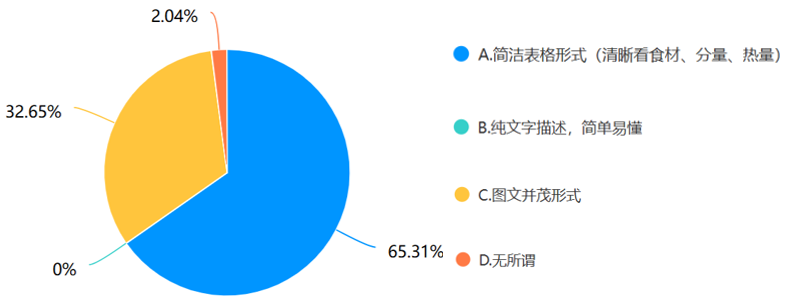
\includegraphics[width=\linewidth]{images/调查者食谱输出形式偏好.png}
    \caption{食谱输出形式偏好}
  \end{subfigure}\hfill
  \begin{subfigure}[b]{0.48\linewidth}
    \centering
    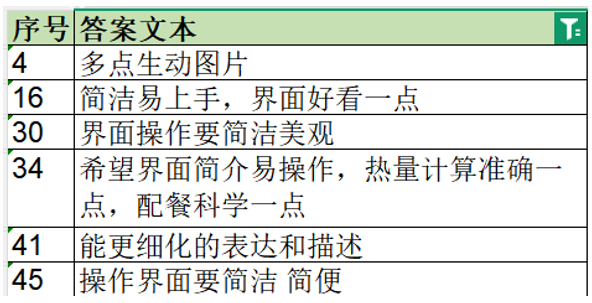
\includegraphics[width=\linewidth]{images/主观题中有关界面的建议.png}
    \caption{主观题中有关界面的建议}
  \end{subfigure}
  \caption{用户界面相关调研反馈}
  \label{fig:ui_survey}
\end{figure}

\item \textbf{整体设计风格}

\begin{subbullet}
\item 整体采用\textbf{清新健康轻量化}的设计语言，以低饱和度薄荷绿作为主品牌色，传递健康、温和、科学的感受；
\item 统一使用\textbf{圆角卡片}与充足留白，减轻用户长时间浏览营养数据带来的视觉压力；
\item 统一使用无衬线字体，建立\textbf{多层字号字重}，突出热量、蛋白质等关键数值，弱化次要说明，保证信息层级清晰。
\end{subbullet}

\item \textbf{整体布局与核心面板}

界面为单页集成式三栏布局（左会话管理栏、中主对话栏、右图标栏 + 工具面板抽屉），仿主流大模型客户端，白底配品牌绿（\texttt{\#4a7c59}）。前端定位为「渲染器」：展示什么内容、以何种形态展示（餐卡 / 食材清单 / 当前规划 / 膳食报告），一律由智能体输出契约（结构化 JSON Schema）决定，前端不预设业务逻辑。

\begin{itemize}[leftmargin=0em, itemsep=1pt, topsep=1pt]
\item \textbf{左·会话管理栏}：Logo、新建对话、历史会话列表、个人档案入口。
\item \textbf{中·主对话栏}：对话流（智能体回复内嵌食谱卡片）+ 底部快捷提示词 + 输入框。
\item \textbf{右·工具栏}：图标竖栏四入口（食材清单 / 当前规划 / 历史方案 / 膳食报告），点击展开抽屉面板；四面板为智能体结构化输出的收集器，只读展示，空态引导回对话发起配餐。
\end{itemize}

\begin{itemize}[leftmargin=0em, itemsep=1pt, topsep=1pt]
\item \textbf{食谱卡片}：状态标签（\texttt{draft} / \texttt{candidates} / \texttt{fixed}）+ 餐次行 +「换一换」+「确认/固定」；支持单餐视图与多日视图，点开查看详细食谱。
\item \textbf{轻量档案弹窗}：身体参数键值 + 胶囊标签（健康目标 / 过敏 / 疾病 / 宗教伦理 / 烹饪设备），支持自定义选项，可随对话补录。
\item \textbf{快捷提示词}：生成一日三餐 / 生成一周食谱 / 推荐一餐搭配 / 生成周膳食报告 / 生成月膳食报告。
\end{itemize}

\begin{figure}[H]
  \centering
  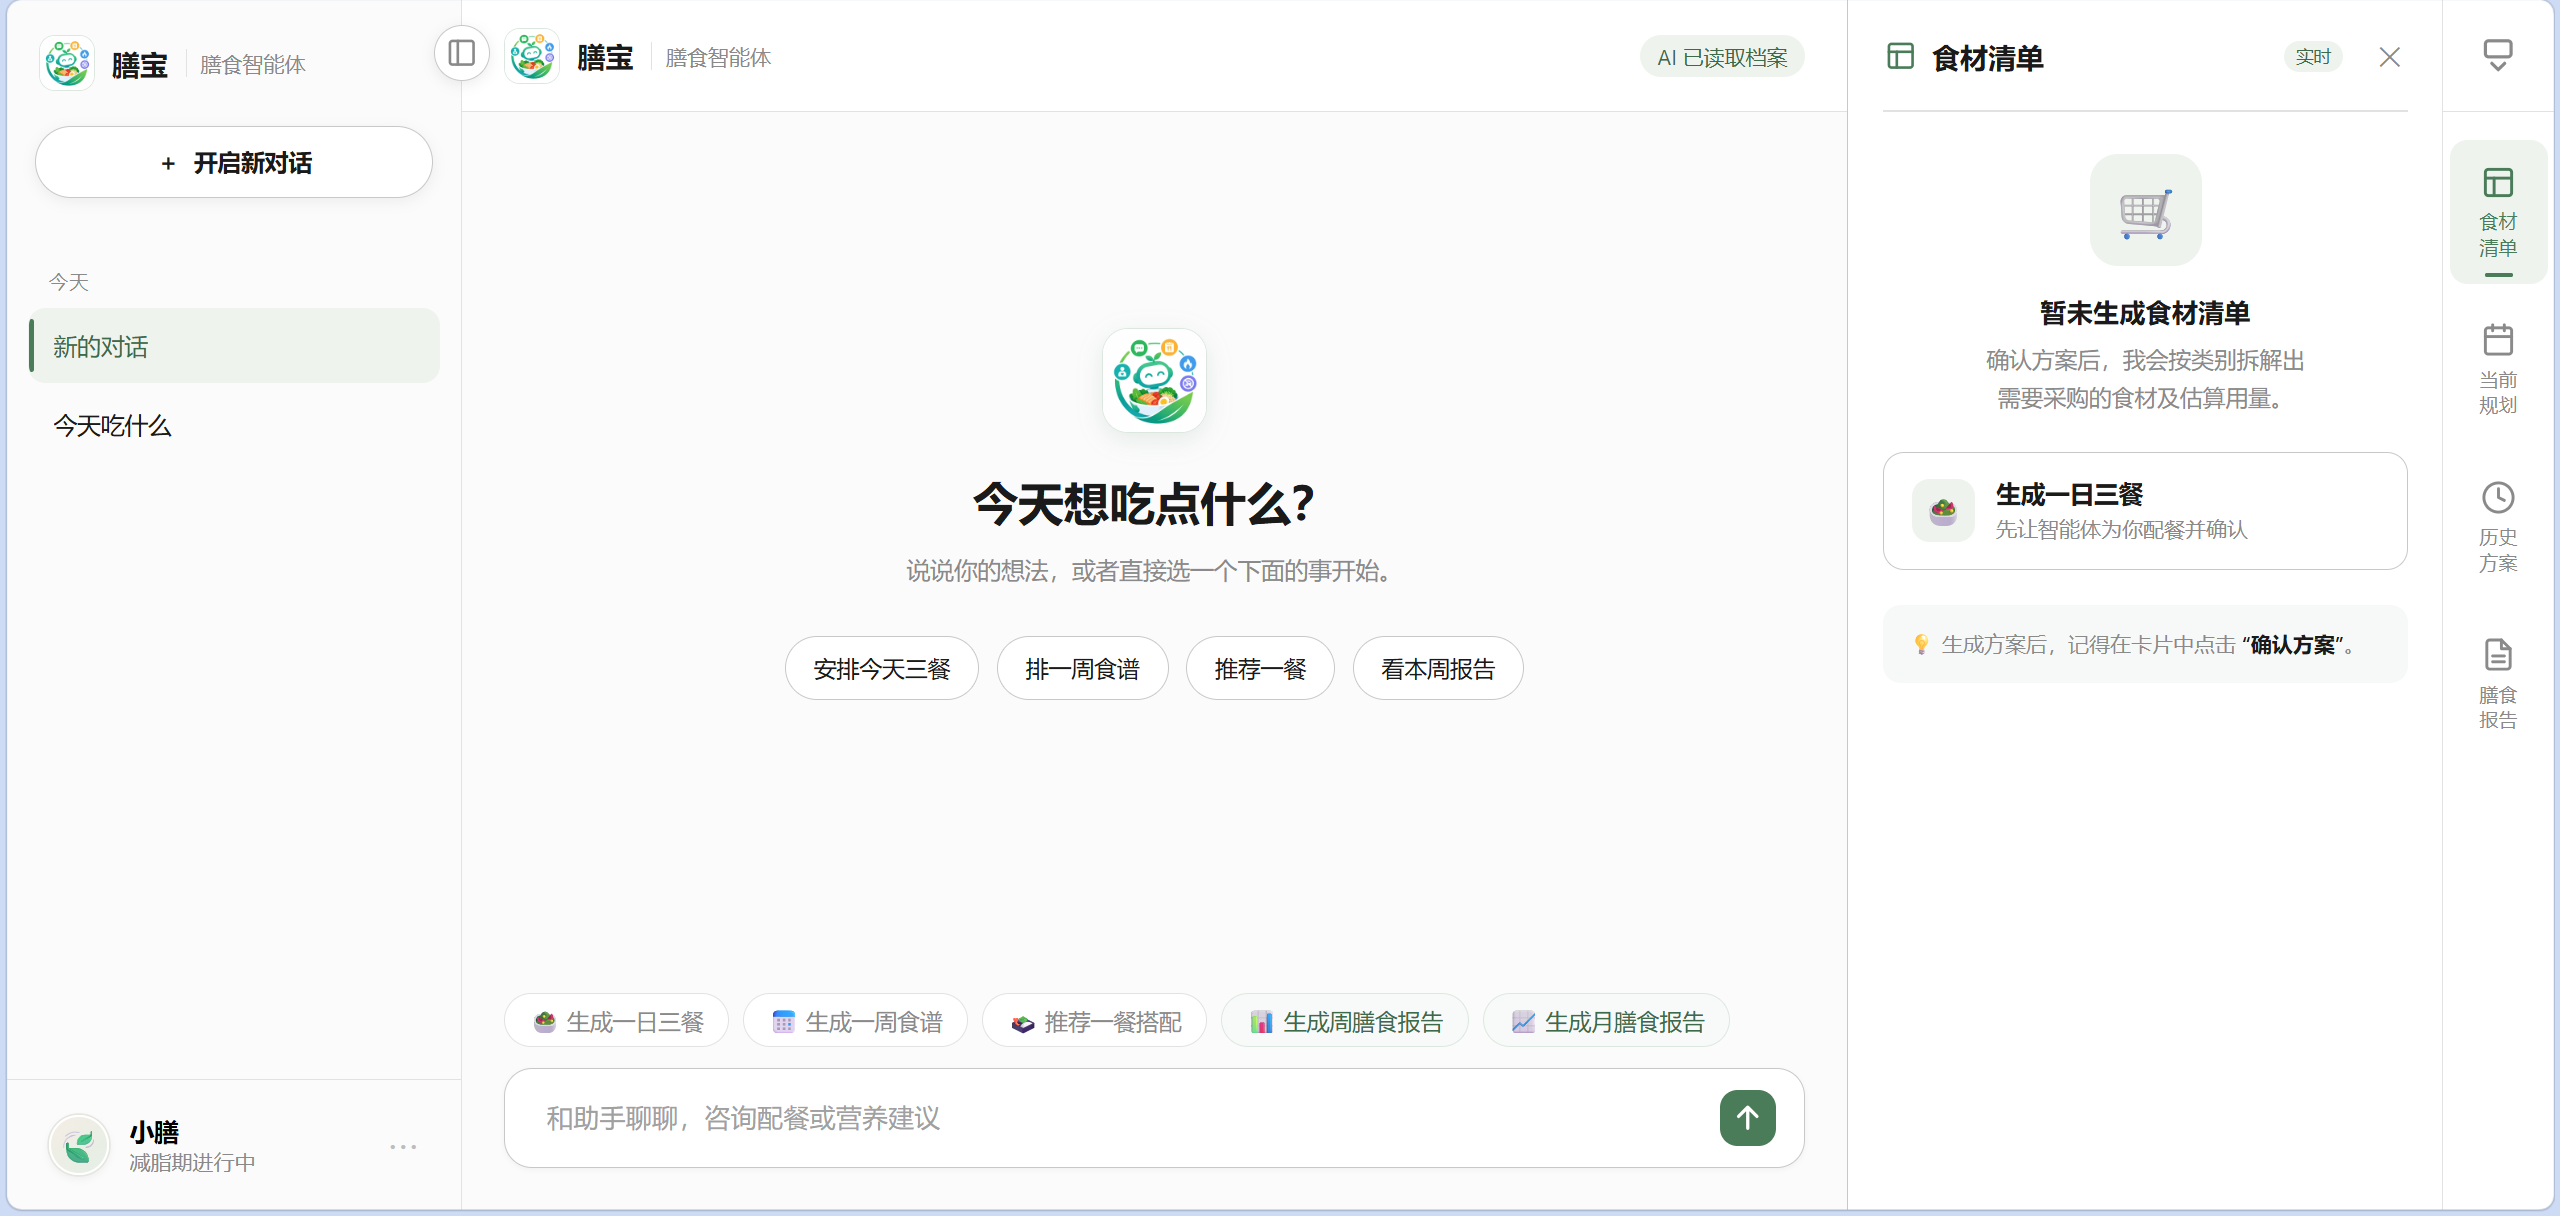
\includegraphics[width=1.0\textwidth]{images/原型.png}
  \caption{系统主界面原型（三栏布局 + 右侧工具面板）}
  \label{fig:prototype}
\end{figure}

\item \textbf{异常情况考量}

针对配餐与交互过程中可能出现的异常，界面与系统统一遵循“不暴露错误、不编造数据、不中断流程、不越过安全边界”的兜底原则：

\begin{enumerate}[label=(\arabic*), leftmargin=10pt, itemsep=2pt, topsep=2pt]
\item \textbf{结构化输出失败}：智能体结果不符合 JSON Schema 时，自动校验并重试，最多 3 次；仍失败则降级为友好提示（如“生成失败，请稍后重试”），不向用户暴露原始错误，也不渲染空白结果。
\item \textbf{数据缺失}：关键营养数据缺失时，不拿 0 顶替、不默认安全，界面以“需核查”标注对应字段，避免把“缺数据”误算成“没营养”。
\item \textbf{检索失败兜底}：知识库检索无结果或异常时，回退到静态规则解释，保证基本配餐流程不中断。
\item \textbf{安全边界}：禁忌规避为硬约束，过敏 / 慢病禁忌食材强制排除并醒目提示；反向营养仅采用“可能 / 建议关注”等非确定性措辞，症状持续时提示及时就医，并在界面明示“不构成医疗诊断”。
\item \textbf{外部服务不可用}：大模型服务超时或不可用时，前端友好提示“服务暂时不可用，请稍后重试”，并保留已生成内容，不丢弃用户进度。
\end{enumerate}

\end{enumerate}

\subsubsection{软件接口}

系统以 RESTful API 对外提供软件接口，所有接口统一返回 JSON（结构须符合~\ref{sec:design-constraints} 结构化输出约束），\texttt{user\_id} 由鉴权注入。以下路径均省略 \path{/api/} 前缀；请求 / 响应体字段定义见第~\ref{sec:data-model}~章数据模型：

\begin{figure}[H]
  \centering
  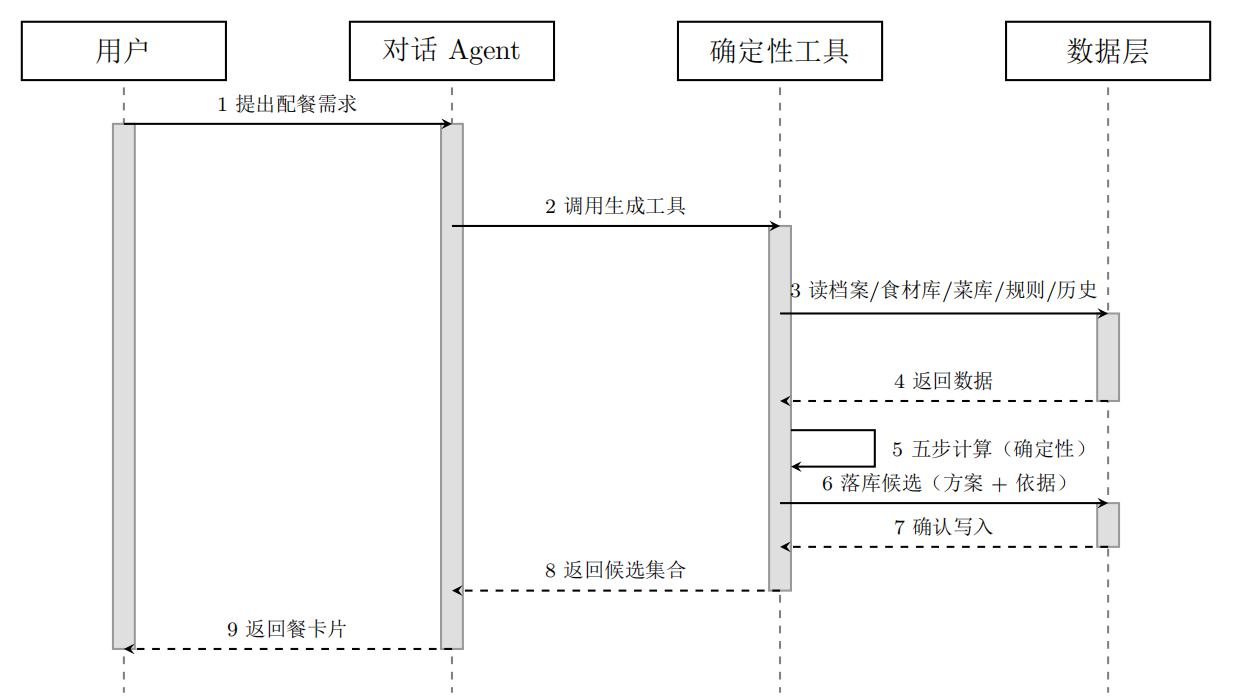
\includegraphics[width=\textwidth]{images/时序图.png}
  \caption{一次配餐请求的交互时序图}
  \label{fig:sequence}
\end{figure}

一次配餐请求的端到端交互时序见图~\ref{fig:sequence}：后端收到请求后先读取用户档案（个人体征、饮食偏好与禁忌），连同请求一起转发给智能体；智能体借大模型识别意图（Function Calling），从内部数据层查询数值基准（关系表）与语义检索知识（向量 RRF），并完成确定性计算，最后把确定性数值带回大模型生成自然语言方案——体现「数值由系统确定性计算给出、大模型不编造」这一设计要点。

{\small\setlength{\tabcolsep}{4pt}
\begin{xltabular}{\linewidth}{P{1.2cm}>{\raggedright\arraybackslash}p{3.5cm}>{\raggedright\arraybackslash}p{3cm}LL}
\caption{软件接口清单} \\
\toprule
\textbf{编号} & \textbf{接口} & \textbf{目的} & \textbf{主要输入} & \textbf{主要输出} \\
\midrule
\endfirsthead
\toprule
\textbf{编号} & \textbf{接口} & \textbf{目的} & \textbf{主要输入} & \textbf{主要输出} \\
\midrule
\endhead
API-01 & GET / PUT \path{/profile} & 读取 / 更新用户档案 & 档案字段集（user\_id 由鉴权注入） & 档案对象（Profile） \\
API-02 & POST \path{/meal-plan/week/generate} & 生成方案（用户自定范围） & 用户消息、目标范围 & MealPlan（状态 draft）：餐位 + 候选 \\
API-03 & POST \path{/meal-plan/candidate/swap} & 同餐换候选并局部重算 & plan\_id、餐位、候选 & 更新后的候选与营养数值 \\
API-04 & POST \path{/meal-plan/week/fix} & 固定方案（锁定选中候选） & plan\_id、选中候选 & MealPlan（状态 fixed） \\
API-05 & GET \path{/meal-plan/current} & 获取当前规划 & user\_id & 当前方案（餐位 / 候选 / 选中） \\
API-06 & GET \path{/meal-plan/{plan_id}} & 获取单份方案详情 & plan\_id & MealPlan 对象 \\
API-07 & GET \path{/meal-plan/list} & 获取历史方案列表 & user\_id、分页参数 & MealPlan 列表 \\
API-08 & POST \path{/nutrition/analysis} & 营养分析（计算并落库） & meal\_plan\_id & 7 关键微量跨日平衡结果 \\
API-09 & GET \path{/nutrition/report} & 获取膳食报告 & meal\_plan\_id & 周 / 月营养复盘报告 \\
API-10 & GET \path{/shopping-list} & 获取食材清单 & meal\_plan\_id & 按分类聚合的采购清单 \\
API-11 & POST \path{/agent/chat} & 与营养智能体多轮对话（SSE） & 用户消息、user\_id、会话 ID & 流式回复（事件 message / done / error） \\
API-12 & POST \path{/agent/rag-query} & RAG 知识库检索 & 查询语句 & 膳食指南 / 食物成分表片段及出处 \\
API-13 & POST \path{/agent/reverse-nutrition} & 反向营养推理（症状$\rightarrow$营养素） & 症状描述文本、user\_id & 可能缺乏的营养素、富含食物建议、就医提示 \\
\bottomrule
\end{xltabular}
}

\noindent 说明：流式输出接口（API-11）的首字延迟要求见~\ref{sec:performance}。

\subsection{系统特征}\label{sec:features}

\begin{figure}[htbp]
  \centering
  \resizebox{\linewidth}{!}{%
  \begin{tikzpicture}[
    font=\small,
    root/.style={draw,rounded corners=3pt,fill=teal!30,align=center,minimum width=3.2cm,minimum height=1.05cm,font=\small\bfseries},
    mod/.style={draw,rounded corners=3pt,fill=teal!10,align=center,text width=5.2cm,minimum height=0.95cm,font=\small},
    leaf/.style={draw,rounded corners=3pt,align=center,text width=5.6cm,inner sep=4pt,font=\small},
    base/.style={leaf,fill=teal!12},
    cond/.style={leaf,dashed,fill=gray!4},
  ]
    % 叶子（链式定位；组内 0.3cm，组间 0.7cm）
    \node[base] (f01) at (0,0)      {\textbf{3.2.1 个人健康档案管理}\\[-1pt]{\scriptsize FR-01\textasciitilde{}03\hspace{1em}基本}};
    \node[base, below=0.3cm of f01] (f02) {\textbf{3.2.2 智能体对话与意图路由}\\[-1pt]{\scriptsize FR-04\textasciitilde{}05\hspace{1em}基本}};
    \node[base, below=0.3cm of f02] (f03) {\textbf{3.2.3 历史方案}\\[-1pt]{\scriptsize FR-06\textasciitilde{}07\hspace{1em}基本}};
    \node[base, below=0.7cm of f03] (f04) {\textbf{3.2.4 个性化能量目标}\\[-1pt]{\scriptsize FR-08\textasciitilde{}10\hspace{1em}基本}};
    \node[base, below=0.3cm of f04] (f05) {\textbf{3.2.5 候选生成与方案调整}\\[-1pt]{\scriptsize FR-11\textasciitilde{}12\hspace{1em}基本}};
    \node[base, below=0.3cm of f05] (f06) {\textbf{3.2.6 营养素配比}\\[-1pt]{\scriptsize FR-13\textasciitilde{}15\hspace{1em}基本}};
    \node[base, below=0.3cm of f06] (f07) {\textbf{3.2.7 家常菜推荐}\\[-1pt]{\scriptsize FR-16\textasciitilde{}18\hspace{1em}基本}};
    \node[base, below=0.3cm of f07] (f08) {\textbf{3.2.8 热量与营养素估算}\\[-1pt]{\scriptsize FR-19\textasciitilde{}21\hspace{1em}基本}};
    \node[base, below=0.3cm of f08] (f09) {\textbf{3.2.9 饮食禁忌提醒}\\[-1pt]{\scriptsize FR-22\textasciitilde{}23\hspace{1em}基本}};
    \node[base, below=0.3cm of f09] (f10) {\textbf{3.2.10 膳食报告}\\[-1pt]{\scriptsize FR-24\textasciitilde{}25\hspace{1em}基本}};
    \node[base, below=0.7cm of f10] (f11) {\textbf{3.2.11 营养原理解释}\\[-1pt]{\scriptsize FR-26\textasciitilde{}27\hspace{1em}基本}};
    \node[cond, below=0.3cm of f11] (f12) {\textbf{3.2.12 反向营养咨询}\\[-1pt]{\scriptsize FR-28\textasciitilde{}30\hspace{1em}有条件}};

    % 模块（各自叶子组的垂直中点，左移 6.8cm）
    \node[mod] (m1) at ($(f01)!0.5!(f03) - (6.8cm,0)$) {人机交互与档案管理};
    \node[mod] (m2) at ($(f04)!0.5!(f10) - (6.8cm,0)$) {智能生成个性化营养膳食方案};
    \node[mod] (m3) at ($(f11)!0.5!(f12) - (6.8cm,0)$) {咨询与原理解释};

    % 根（模块垂直中点，再左移 6.0cm，与模块之间留约 1.6cm 间隙）
    \node[root] (root) at ($(m1)!0.5!(m3) - (6.0cm,0)$) {膳食搭配智能体系统\\[2pt] {\scriptsize（3.2 系统特征）}};

    % 连线：根 → 模块
    \draw[->] (root.east) -- (m1.west);
    \draw[->] (root.east) -- (m2.west);
    \draw[->] (root.east) -- (m3.west);

    % 连线：模块 → 特征
    \draw[->] (m1.east) -- (f01.west);
    \draw[->] (m1.east) -- (f02.west);
    \draw[->] (m1.east) -- (f03.west);
    \draw[->] (m2.east) -- (f04.west);
    \draw[->] (m2.east) -- (f05.west);
    \draw[->] (m2.east) -- (f06.west);
    \draw[->] (m2.east) -- (f07.west);
    \draw[->] (m2.east) -- (f08.west);
    \draw[->] (m2.east) -- (f09.west);
    \draw[->] (m2.east) -- (f10.west);
    \draw[->] (m3.east) -- (f11.west);
    \draw[->] (m3.east) -- (f12.west);
  \end{tikzpicture}}

  \par\medskip
  {\footnotesize
   
\begin{tikzpicture}[baseline=-0.6ex]
     \node[draw,rounded corners=2pt,fill=teal!12,inner sep=0pt,minimum width=1.1em,minimum height=0.9em]{};
   \end{tikzpicture}\;\;基本（MVP，本阶段实现）\hspace{3em}
   \begin{tikzpicture}[baseline=-0.6ex]
     \node[draw,dashed,rounded corners=2pt,fill=white,inner sep=0pt,minimum width=1.1em,minimum height=0.9em]{};
   \end{tikzpicture}\;\;有条件（视进度实现）}

  \caption{系统功能树：三大模块 $\rightarrow$ 12 个特征 $\rightarrow$ 功能需求（FR）}
  \label{fig:feature-tree}
\end{figure}

系统各特征的需求说明如下：

\begin{enumerate}
\item \textbf{个人健康档案管理}
  \begin{enumerate}[label=(\arabic*), leftmargin=10pt, itemsep=2pt, topsep=2pt]
    \item \textbf{目的：}一次性采集并持久化用户个体化信息，供后续每次配餐与咨询自动读取；作为所有个性化计算与硬约束过滤的统一输入基础。
    \item \textbf{激励/响应序列}
      \begin{itemize}[leftmargin=*, itemsep=1pt, topsep=1pt]
        \item \textbf{激励（输入）}：性别、年龄、身高、体重、健康目标、烹饪设备、疾病、过敏、宗教伦理禁忌、口味偏好；
        \item \textbf{响应（输出）}：档案对象（含 \texttt{user\_id}），持久化并可被后续请求自动读取。
      \end{itemize}
    \item \textbf{相关功能需求}
      \begin{itemize}[leftmargin=*, itemsep=1pt, topsep=1pt]
        \item \textbf{FR-01：}系统应支持创建、更新、保存与读取用户个人健康档案；
        \item \textbf{FR-02：}系统应在生成方案或咨询时自动读取当前用户档案，无需重复录入；
        \item \textbf{FR-03：}系统应对身高、体重、疾病、过敏等敏感信息加密存储。
      \end{itemize}
  \end{enumerate}

\item \textbf{智能体对话与意图路由}
  \begin{enumerate}[label=(\arabic*), leftmargin=10pt, itemsep=2pt, topsep=2pt]
    \item \textbf{目的：}以自然语言多轮对话接收请求，经意图路由归入「询问 / 配餐 / 调整」三条路径，降低使用门槛并贯通各项特征。
    \item \textbf{激励/响应序列}
      \begin{itemize}[leftmargin=*, itemsep=1pt, topsep=1pt]
        \item \textbf{激励（输入）}：用户消息 + 会话上下文 + \texttt{user\_id}；
        \item \textbf{响应（输出）}：智能体回复（流式输出）。
      \end{itemize}
    \item \textbf{相关功能需求}
      \begin{itemize}[leftmargin=*, itemsep=1pt, topsep=1pt]
        \item \textbf{FR-04：}系统应支持与营养智能体进行带上下文的多轮对话；
        \item \textbf{FR-05：}系统应将配餐相关请求编排至确定性计算工具（Function Calling），大模型不得直接计算或编造数值。
      \end{itemize}
  \end{enumerate}

\item \textbf{历史方案}
  \begin{enumerate}[label=(\arabic*), leftmargin=10pt, itemsep=2pt, topsep=2pt]
    \item \textbf{目的：}保存历史配餐方案供用户回看与复用，避免重复录入，支撑连续性饮食管理。
    \item \textbf{激励/响应序列}
      \begin{itemize}[leftmargin=*, itemsep=1pt, topsep=1pt]
        \item \textbf{激励（输入）}：\texttt{user\_id}、历史方案查询 / 复用请求；
        \item \textbf{响应（输出）}：历史方案列表、方案详情、复用后的新方案。
      \end{itemize}
    \item \textbf{相关功能需求}
      \begin{itemize}[leftmargin=*, itemsep=1pt, topsep=1pt]
        \item \textbf{FR-06：}系统应保存每次生成的配餐方案并可回看；
        \item \textbf{FR-07：}系统应支持复用历史方案。
      \end{itemize}
  \end{enumerate}

\item \textbf{个性化能量目标}
  \begin{enumerate}[label=(\arabic*), leftmargin=10pt, itemsep=2pt, topsep=2pt]
    \item \textbf{目的：}依据用户档案计算个性化能量目标，仅作份量量级参考（决定吃多少），不做热量缺口或盈余。
    \item \textbf{激励/响应序列}
      \begin{itemize}[leftmargin=*, itemsep=1pt, topsep=1pt]
        \item \textbf{激励（输入）}：性别 / 年龄 / 身高 / 体重 / 健康目标；
        \item \textbf{响应（输出）}：个性化能量目标（kcal）。
      \end{itemize}
    \item \textbf{相关功能需求}
      \begin{itemize}[leftmargin=*, itemsep=1pt, topsep=1pt]
        \item \textbf{FR-08：}系统应依据 Mifflin-St Jeor 公式计算 BMR；
        \item \textbf{FR-09：}系统应以固定活动系数计算能量目标（能量目标 = BMR $\times$ 1.4），仅作份量量级，不做热量缺口 / 盈余；
        \item \textbf{FR-10：}系统应使健康目标只改变结构（宏量供能比 / 油盐糖 / 食材做法倾向）而不改变热量，覆盖维持 / 减脂 / 增肌 / 控糖 / 改善肠胃五类；热量缺口 / 盈余留后期改进。
      \end{itemize}
  \end{enumerate}

\item \textbf{候选生成与方案调整}
  \begin{enumerate}[label=(\arabic*), leftmargin=10pt, itemsep=2pt, topsep=2pt]
    \item \textbf{目的：}从全量食材库确定性生成每餐候选，支持用户「换一换」与「确认 / 固定」，数值一律经确定性工具局部重算。
    \item \textbf{激励/响应序列}
      \begin{itemize}[leftmargin=*, itemsep=1pt, topsep=1pt]
        \item \textbf{激励（输入）}：用户自定生成范围（一餐 / 一日 / 数日 / 一周或更长）+ 档案硬软约束；
        \item \textbf{响应（输出）}：每餐 2\textasciitilde{}3 个候选（含做法与营养），换候选后同步更新数值，固定后方案只读锁定。
      \end{itemize}
    \item \textbf{相关功能需求}
      \begin{itemize}[leftmargin=*, itemsep=1pt, topsep=1pt]
        \item \textbf{FR-11：}系统应经规则引擎五步算法生成候选（算目标 $\rightarrow$ 构造候选 $\rightarrow$ 差异化 $\rightarrow$ 跨日微量平衡 $\rightarrow$ 输出）；每餐 = 主食 + 1\textasciitilde{}2 道菜，靠换主食材 / 换做法差异化；过敏 / 疾病 / 宗教禁忌硬排除、个人偏好软排除；
        \item \textbf{FR-12：}系统应支持「换一换」与「确认 / 固定」，方案状态机为 draft（生成中）$\rightarrow$ candidates（候选可换）$\rightarrow$ fixed（已固定只读锁定），换候选经确定性工具局部重算并同步营养数值。
      \end{itemize}
  \end{enumerate}

\item \textbf{营养素配比（宏量按餐、关键微量跨日动态平衡）}
  \begin{enumerate}[label=(\arabic*), leftmargin=10pt, itemsep=2pt, topsep=2pt]
    \item \textbf{目的：}以“营养素配比平衡”为核心，输出宏量营养素（按餐）目标，7 种关键微量营养素跨日动态平衡，区别于一般热量计算器。
    \item \textbf{激励/响应序列}
      \begin{itemize}[leftmargin=*, itemsep=1pt, topsep=1pt]
        \item \textbf{激励（输入）}：个性化能量目标 + 硬约束（疾病 / 过敏 / 禁忌、油盐糖上限）+ 近期历史方案；
        \item \textbf{响应（输出）}：每餐宏量配比目标（早 30\% / 中 40\% / 晚 30\%）+ 7 种关键微量跨日平衡目标。
      \end{itemize}
    \item \textbf{相关功能需求}
      \begin{itemize}[leftmargin=*, itemsep=1pt, topsep=1pt]
        \item \textbf{FR-13：}系统应按供能比计算宏量营养素配比（碳水 50\textasciitilde{}65\%、脂肪 20\textasciitilde{}30\%、蛋白 10\textasciitilde{}20\%）并按三餐分配（早 30\% / 午 40\% / 晚 30\%，可调）；
        \item \textbf{FR-14：}系统应叠加疾病、过敏、禁忌等硬约束及油盐糖上限；
        \item \textbf{FR-15：}系统应对 7 种关键微量（钙、铁、锌、维 A、B1、B2、C）做跨日动态平衡，读取近期历史方案识别不足并回溯补位；钠归「油盐糖」控制、膳食纤维归「宏量结构」，其余微量仅作参考提示。
      \end{itemize}
  \end{enumerate}

\item \textbf{家常菜推荐（菜式落地）}
  \begin{enumerate}[label=(\arabic*), leftmargin=10pt, itemsep=2pt, topsep=2pt]
    \item \textbf{目的：}将第一步的食材清单转化为可购买、可制作的家常菜，给出烹饪方式与油盐估算，解决“营养清单到现实餐食”的落地问题（现阶段聚焦自行烹饪）。
    \item \textbf{激励/响应序列}
      \begin{itemize}[leftmargin=*, itemsep=1pt, topsep=1pt]
        \item \textbf{激励（输入）}：食材清单 + 初步热量 + 禁忌过滤条件 + 口味偏好；
        \item \textbf{响应（输出）}：家常菜菜单（含烹饪方式与油盐分级估算）。
      \end{itemize}
    \item \textbf{相关功能需求}
      \begin{itemize}[leftmargin=*, itemsep=1pt, topsep=1pt]
        \item \textbf{FR-16：}系统应从家常菜库按每餐营养目标匹配菜式并给出烹饪方式与步骤；
        \item \textbf{FR-17：}系统应优先推荐清蒸、凉拌等低油做法；
        \item \textbf{FR-18：}系统应支持换候选时生成同营养替代菜品建议（排除某食材 / 更换做法）。
      \end{itemize}
  \end{enumerate}

\item \textbf{热量与营养素估算（双口径）}
  \begin{enumerate}[label=(\arabic*), leftmargin=10pt, itemsep=2pt, topsep=2pt]
    \item \textbf{目的：}自动给出每餐、全天热量与三大营养素数值，并明确区分“食材口径”与“菜式口径”两套热量含义，避免用户混淆。
    \item \textbf{激励/响应序列}
      \begin{itemize}[leftmargin=*, itemsep=1pt, topsep=1pt]
        \item \textbf{激励（输入）}：食材列表（生重）或菜式列表（含做法、份量）；
        \item \textbf{响应（输出）}：食材口径热量、菜式口径热量、三大营养素（克）。
      \end{itemize}
    \item \textbf{相关功能需求}
      \begin{itemize}[leftmargin=*, itemsep=1pt, topsep=1pt]
        \item \textbf{FR-19：}系统应按《中国食物成分表》口径计算食材（生重）热量与营养素；
        \item \textbf{FR-20：}系统应在菜式口径叠加烹饪油盐估算热量（1 g 油脂 $\approx$ 9 kcal），并与食材口径分别标注；
        \item \textbf{FR-21：}系统应以低 / 中 / 高分级结合克数区间估算油盐，不得输出伪精确的单一克数。
      \end{itemize}
  \end{enumerate}

\item \textbf{饮食禁忌提醒（硬约束过滤）}
  \begin{enumerate}[label=(\arabic*), leftmargin=10pt, itemsep=2pt, topsep=2pt]
    \item \textbf{目的：}自动规避用户档案标记的过敏食材与慢病不适宜食材并给出提示，保障饮食安全。
    \item \textbf{激励/响应序列}
      \begin{itemize}[leftmargin=*, itemsep=1pt, topsep=1pt]
        \item \textbf{激励（输入）}：用户档案（过敏、疾病、禁忌）+ 候选菜式；
        \item \textbf{响应（输出）}：过滤后的菜式 + 禁忌依据说明。
      \end{itemize}
    \item \textbf{相关功能需求}
      \begin{itemize}[leftmargin=*, itemsep=1pt, topsep=1pt]
        \item \textbf{FR-22：}系统应将疾病、过敏、禁忌设为硬约束，在推荐菜式时自动过滤（如糖尿病规避高 GI、高血压限盐）；
        \item \textbf{FR-23：}系统应对被规避的菜式给出提醒及依据说明。
      \end{itemize}
  \end{enumerate}

\item \textbf{膳食报告（周 / 月复盘）}
  \begin{enumerate}[label=(\arabic*), leftmargin=10pt, itemsep=2pt, topsep=2pt]
    \item \textbf{目的：}汇总已确认方案的营养摄入，输出周 / 月膳食报告与后续调整建议，数据不完整时标注缺失。
    \item \textbf{激励/响应序列}
      \begin{itemize}[leftmargin=*, itemsep=1pt, topsep=1pt]
        \item \textbf{激励（输入）}：\texttt{user\_id}、报告周期；
        \item \textbf{响应（输出）}：周 / 月营养摄入汇总、RNI 对照、不足 / 过量项、数据缺失标注与调整建议。
      \end{itemize}
    \item \textbf{相关功能需求}
      \begin{itemize}[leftmargin=*, itemsep=1pt, topsep=1pt]
        \item \textbf{FR-24：}系统应汇总已确认方案营养摄入，生成周 / 月膳食报告，标注不足 / 过量项与数据缺失；
        \item \textbf{FR-25：}系统应给出后续饮食调整建议。
      \end{itemize}
  \end{enumerate}

\item \textbf{营养原理解释}
  \begin{enumerate}[label=(\arabic*), leftmargin=10pt, itemsep=2pt, topsep=2pt]
    \item \textbf{目的：}解释“为何如此搭配”及营养素的生理作用，降低非专业用户的理解门槛。
    \item \textbf{激励/响应序列}
      \begin{itemize}[leftmargin=*, itemsep=1pt, topsep=1pt]
        \item \textbf{激励（输入）}：配餐方案 / 用户提问 + RAG 检索结果；
        \item \textbf{响应（输出）}：配餐依据与营养原理说明，附权威来源。
      \end{itemize}
    \item \textbf{相关功能需求}
      \begin{itemize}[leftmargin=*, itemsep=1pt, topsep=1pt]
        \item \textbf{FR-26：}系统应结合知识库解释配餐依据与营养素生理作用；
        \item \textbf{FR-27：}系统应对关键结论标注权威来源（《中国居民膳食指南（2022）》《中国食物成分表》等），可核实、可溯源。
      \end{itemize}
  \end{enumerate}

\item \textbf{反向营养咨询（有条件）}
  \begin{enumerate}[label=(\arabic*), leftmargin=10pt, itemsep=2pt, topsep=2pt]
    \item \textbf{目的：}由用户描述的身体症状推测可能缺乏的营养素并给出膳食建议，作为区别于通用计算器的反向推理能力；本阶段仅作「推测 + 就医提示」，不做确定性医学推理（见尚待解决 P1）。
    \item \textbf{激励/响应序列}
      \begin{itemize}[leftmargin=*, itemsep=1pt, topsep=1pt]
        \item \textbf{激励（输入）}：症状描述文本 + 用户档案；
        \item \textbf{响应（输出）}：可能缺乏的营养素 + 富含该营养素的食物 + 就医提示。
      \end{itemize}
    \item \textbf{相关功能需求}
      \begin{itemize}[leftmargin=*, itemsep=1pt, topsep=1pt]
        \item \textbf{FR-28：}系统应基于“症状---营养素”知识库推测可能缺乏的营养素；
        \item \textbf{FR-29：}系统应使用“可能 / 建议关注”等非确定性措辞，不得给出诊断性结论；
        \item \textbf{FR-30：}系统应在回复末尾提示“若症状持续请及时就医”，并声明不替代医学诊断。
      \end{itemize}
  \end{enumerate}
\end{enumerate}

\subsection{性能需求}\label{sec:performance}

系统性能需求以可测量的指标规定如下：

\begin{xltabular}{\linewidth}{Lp{4.5cm}}
\caption{系统性能需求指标} \\
\toprule
\textbf{性能指标} & \textbf{目标值} \\
\midrule
\endfirsthead
\toprule
\textbf{性能指标} & \textbf{目标值} \\
\midrule
\endhead
配餐生成响应（含 LLM 推理与两步模型编排） & P95 $\leq$ 15 秒 \\
确定性计算接口（BMR $\times$ 1.4 / 营养核算 / 候选生成 / 跨日微量回溯） & P99 $\leq$ 100 毫秒 \\
数据库查询（食材库、家常菜库关键词搜索） & P95 $\leq$ 1 秒 \\
档案读写（读取与保存） & P95 $\leq$ 500 毫秒 \\
膳食报告（汇总已确认方案营养生成评估） & P95 $\leq$ 3 秒 \\
智能体对话首字延迟（流式输出） & $\leq$ 10 秒 \\
反向营养推理（症状 $\rightarrow$ 营养素推测，含知识库检索与 LLM 生成） & P95 $\leq$ 15 秒 \\
RAG 知识检索（膳食指南 / 食物成分表 Top-K 片段） & P95 $\leq$ 2 秒 \\
并发能力（同时在线用户） & $\geq$ 50 用户 \\
结构化输出成功率（一次通过 JSON Schema 校验） & $\geq$ 95\% \\
\bottomrule
\end{xltabular}

\begin{quote}
注：P95 / P99 表示相应百分位的请求须满足目标值；智能体对话首字延迟为流式输出的绝对上限。
\end{quote}

\subsection{设计约束}\label{sec:design-constraints}

系统设计须遵循以下约束：

\begin{enumerate}
\item \textbf{标准依从性}：营养素数据统一采用《中国食物成分表（标准版）》口径；推荐与配比依据《中国居民膳食指南（2022）》及《中国居民膳食营养素参考摄入量（2023版）》，所有营养建议须标注所依据的标准或权威来源。
\item \textbf{确定性计算约束}：BMR、能量目标、热量核算、宏量营养素配比、三餐分配、候选生成、跨日微量平衡等所有数值计算必须由后端确定性工具完成，大模型不得直接计算或编造数值。
\item \textbf{结构化输出约束}：智能体的配餐结果输出必须符合预定义的 JSON Schema，前端方可稳定解析；结构化校验失败时自动重试，最多 3 次，仍失败则返回降级提示。
\item \textbf{技术接口约束}：所选大模型必须支持 Function Calling 与 JSON 结构化输出（structured output）能力，不满足者不得接入；食材数据依赖结构化成分数据库。
\item \textbf{Agent 行为铁律}：零编造 / null $\neq$ 0 / data\_quality 三态语义 / 未核查 $\neq$ 安全 / 可溯源 / 硬约束优先 / needs\_clarification 必须追问 / 不做医学诊断。
\end{enumerate}

\subsection{软件系统属性}\label{sec:attributes}

\begin{enumerate}
\item \textbf{安全保密性}
  \begin{subbullet}
  \item \textbf{具体要求}：用户身高、体重、疾病、过敏、禁忌等身体数据属个人敏感信息，存储时加密；仅用于本系统生成膳食方案，不向任何第三方提供或共享；数据采集遵循最小必要原则。
  \item \textbf{可验证方式}：抽查数据库字段是否加密、接口是否有越权访问漏洞。
  \end{subbullet}
\item \textbf{可靠性}
  \begin{subbullet}
  \item \textbf{具体要求}：确定性计算结果可复现；LLM API 不可用时档案浏览与历史方案仍可访问（确定性计算与结构化输出的具体规则见~\ref{sec:design-constraints}）。
  \item \textbf{可验证方式}：模拟 LLM 返回非法 JSON，观察重试与降级行为；同一档案多次计算结果一致。
  \end{subbullet}
\item \textbf{可用性}
  \begin{subbullet}
  \item \textbf{具体要求}：核心配餐流程在 3 步内完成（填档案 $\rightarrow$ 生成方案 $\rightarrow$ 查看结果）；界面语言通俗，不具备营养学背景的普通用户可独立使用；油盐用量以分级形式呈现，易于理解。
  \item \textbf{可验证方式}：新用户无引导下完成一次配餐的任务测试。
  \end{subbullet}
\item \textbf{可维护性}
  \begin{subbullet}
  \item \textbf{具体要求}：食材库、家常菜库、知识库内容可通过后台独立更新，无需修改业务代码；规则引擎、智能体 Prompt 与 JSON Schema 版本可追溯。
  \item \textbf{可验证方式}：后台更新一条食材数据后，配餐结果中对应数值即时变化。
  \end{subbullet}
\item \textbf{可解释性}
  \begin{subbullet}
  \item \textbf{具体要求}：所有营养建议均标注权威来源（膳食指南、食物成分表）；关键计算（BMR、营养素配比）过程可追溯；智能体回复说明配餐依据与营养原理（详细解释见 3.2.11）。
  \item \textbf{可验证方式}：抽查配餐方案页与对话回复，确认是否标注来源、是否说明依据。
  \end{subbullet}
\item \textbf{可扩展性}
  \begin{subbullet}
  \item \textbf{具体要求}：两步模型架构支持平滑扩展：家常菜库可扩充至食堂/外卖常见菜式；微量营养素可从核心项扩展至全谱。
  \item \textbf{可验证方式}：新增一道菜式后无需修改核心代码即可被配餐系统调用。
  \end{subbullet}
\item \textbf{可移植性}
  \begin{subbullet}
  \item \textbf{具体要求}：系统为纯 Web 应用，基于标准浏览器访问、无需客户端安装，可在主流浏览器（Chrome、Edge、Safari）及常见桌面/移动设备上运行；服务端采用通用技术栈，可在轻量服务器上部署，无专用硬件依赖。
  \item \textbf{可验证方式}：在不同浏览器与设备上打开系统完成一次配餐流程，功能与排版正常。
  \end{subbullet}
\end{enumerate}

\section{数据/对象模型}\label{sec:data-model}

本章给出系统核心领域对象及其关系，作为数据库设计与智能体数据结构的依据（详细设计见概要设计 DBDD）。系统的逻辑数据需求如下：

\begin{enumerate}
\item \textbf{核心实体（业务侧，app schema）}：用户档案（Profile）、膳食方案（MealPlan）、餐位（MealSlot）、候选（MealCandidate）、候选菜品（MealCandidateDish）、食材清单（ShoppingList）、营养报告（NutritionReport）、会话（Conversation）、消息（Message）。
\item \textbf{权威字典（core schema，只读）}：食材（Ingredient）、菜式（Dish）、菜式配方（Recipe）、营养素参考值（NutritionReference）、疾病规则。
\item \textbf{知识（knowledge schema，只读）}：膳食指南 / 成分表 / DRIs 知识条目，供 RAG 检索。
\item \textbf{四级方案状态机}：MealPlan $1$---$*$ MealSlot $1$---$*$ MealCandidate $1$---$*$ MealCandidateDish；方案状态 \texttt{draft}（生成中）$\rightarrow$ \texttt{candidates}（候选可换）$\rightarrow$ \texttt{fixed}（已固定只读锁定）。
\item \textbf{四 Schema 与权限}：\texttt{core}（权威数值，只读）/ \texttt{knowledge}（知识，只读）/ \texttt{app}（业务，读写）/ \texttt{audit}（审核，只增）；应用连接非超级用户，Agent 不直连库、一律经后端。
\item \textbf{数据基线}：128 食材 / 60 菜 / 16 做法规则 / 18 营养素·448 参考值 / 26 知识；\texttt{data\_quality} 三态（official / approx / check）、过敏原三态（含 / 不含 / 未核查）、\texttt{null} 表示未知而非 0。
\item \textbf{数据来源}：营养成分数据来自《中国食物成分表（标准版）》等权威数据源，须结构化入库、可解析、可溯源（见~\ref{sec:constraints}、\hyperref[appendix:b]{附录 B}）。
\end{enumerate}

类之间的关联关系如图~\ref{fig:class} 所示（四级方案状态机与四 Schema 的完整实体关系见概要设计 DBDD）。

\begin{figure}[htbp]
	\centering
	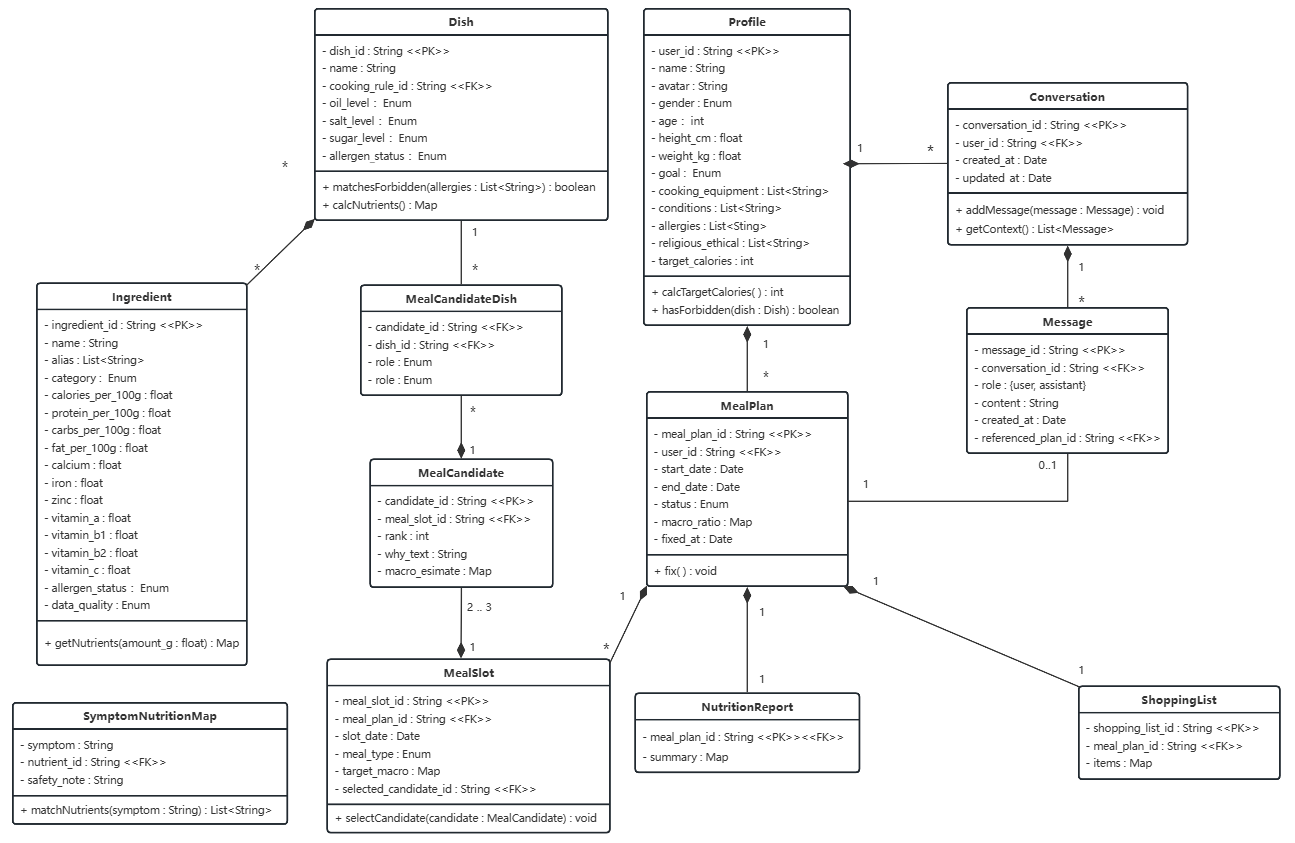
\includegraphics[width=0.85\textwidth]{images/类图.png}
	\caption{核心领域对象类图}
	\label{fig:class}
\end{figure}

\section{验收标准}

\subsection{代表性领域任务}\label{sec:acceptance-tasks}

{\small\begin{xltabular}{\linewidth}{P{1.0cm}Q{2.5cm}Q{2.5cm}Q{3cm}L}
\caption{代表性领域任务与验收条件} \\
\toprule
\textbf{编号} & \textbf{代表性任务} & \textbf{检查方式} & \textbf{覆盖条款} & \textbf{通过条件} \\
\midrule
\endfirsthead
\toprule
\textbf{编号} & \textbf{代表性任务} & \textbf{检查方式} & \textbf{覆盖条款} & \textbf{通过条件} \\
\midrule
\endhead
R-01 & 为“25 岁、160cm、60kg、减脂目标”女性配一日三餐 & 输入档案并运行配餐 & 3.2.4 能量目标、3.2.5 候选、3.2.6 配比、3.2.7 家常菜、3.2.8 热量、3.2.9 禁忌（FR-08\textasciitilde{}23） & 能量目标约 1839.6 kcal（BMR 1314 $\times$ 1.4，仅份量量级、无热量缺口）、每餐 2\textasciitilde{}3 候选、三餐按约 30/40/30 分配、每餐热量与三大营养素，并落地为家常菜（含烹饪方式与油盐分级） \\
R-02 & 创建并复用用户档案 & 填写档案后再次发起配餐 & 3.2.1 档案管理（FR-01\textasciitilde{}03） & 首次填写身高体重、疾病、过敏后，后续配餐自动读取档案、无需重复录入；敏感字段加密存储 \\
R-03 & 为“有糖尿病”用户配餐 & 档案标记糖尿病并运行配餐 & 3.2.9 禁忌提醒（FR-22、FR-23） & 自动规避高 GI 食材、控制碳水比例，并对被规避菜式给出依据说明 \\
R-04 & 询问“米饭的营养成分” & 发起营养查询 & 3.2.8 热量估算、3.2.11 营养原理解释（FR-19、FR-27） & 引用《中国食物成分表》给出准确数值并标注出处 \\
R-05 & 对生成方案“换一换”并确认固定 & 对方案点换一换、确认固定 & 3.2.5 候选生成与方案调整（FR-11、FR-12） & 换候选后营养数值同步更新；方案状态 draft $\rightarrow$ candidates $\rightarrow$ fixed，固定后只读锁定 \\
R-06 & 追问“为什么这样搭配” & 对配餐结果发起解释请求 & 3.2.11 营养原理解释（FR-26、FR-27） & 说明配餐依据与营养素生理作用，关键结论标注权威来源（膳食指南/食物成分表） \\
R-07 & 描述“近期总乏力”，询问可能缺乏什么 & 发起反向营养对话 & 3.2.12 反向营养（FR-28\textasciitilde{}30） & 输出“可能缺乏铁”等推测、依据与食物建议，使用非确定性措辞并附“若症状持续请及时就医”提示 \\
R-08 & 请求“生成周膳食报告” & 输入报告周期并生成报告 & 3.2.10 膳食报告（FR-24、FR-25） & 输出已确认方案的营养汇总、RNI 对照、不足 / 过量与数据缺失标注，并给出后续调整建议 \\
R-09 & 连续多轮对话调整配餐 & 在对话中连续追加条件 & 3.2.2 智能体对话与意图路由（FR-04、FR-05） & 支持带上下文的多轮对话；数值由确定性计算工具（Function Calling）给出，大模型不直接编造数值 \\
R-10 & 回看并复用历史方案 & 查询历史方案并点击复用 & 3.2.3 历史方案（FR-06、FR-07） & 历史方案列表可查；支持一键复用（重新生成或复制食材清单） \\
\bottomrule
\end{xltabular}}

\subsection{定制效果检查方式}

定制效果采用“同一输入、A/B 对比”的方式检查：将下表中同一组输入分别送入未定制的通用大模型与定制智能体，由产品组与测试岗按“验收通过的关键检查点”逐项判定（满足 / 不满足）。通用大模型仅作为定性基线，用于说明定制带来的差异，其输出以模型建成后的实测为准，不作为正式验收项。

{\small\begin{xltabular}{\linewidth}{p{2.0cm}Q{2.8cm}LQ{4.0cm}}
\caption{定制效果检查方式} \\
\toprule
\textbf{测试输入} & \textbf{通用模型常见表现} & \textbf{定制智能体验收标准} & \textbf{验收通过的关键检查点} \\
\midrule
\endfirsthead
\toprule
\textbf{测试输入} & \textbf{通用模型常见表现} & \textbf{定制智能体验收标准} & \textbf{验收通过的关键检查点} \\
\midrule
\endhead
“给我一份减脂食谱” & 泛泛给出通用建议/模板，常忽略具体身高体重数据，热量与宏量分配易偏离 & 自动提取用户档案，按能量目标进行三餐分配，明确标注热量与营养素，并落地为具体家常菜 & \begin{cellenum}\item 是否结合身体数据计算。\item 是否给出精确数值。\item 是否落地为家常菜做法。\end{cellenum} \\
“有糖尿病怎么吃” & 泛泛回答“少吃糖/少吃主食”，忽略整体膳食结构 & 优先选择低 GI 主食，严格控制全天碳水总量，明确给出控制依据并附“非医疗建议”提示 & \begin{cellenum}\item 是否给出低 GI 与控碳水依据。\item 是否附“非医疗建议”提示。\end{cellenum} \\
“米饭营养怎么样” & 直接给出无出处的估算值，重复提问数值可能不一致 & 引用《中国食物成分表》给出可追溯的参考值，并提示受品种与烹饪方式影响 & \begin{cellenum}\item 数值是否标注权威出处。\item 是否说明“参考值”口径及烹饪影响。\end{cellenum} \\
“最近总感觉乏力” & 泛泛建议休息或就医，未结合营养学给出科学归因 & 不作出诊断，列举多种可能因素进行科普，给出富含铁等对应食材建议，并强制附带就医提示 & \begin{cellenum}\item 是否使用“可能”等非确定性措辞。\item 是否给出食物层面的科普建议。\item 是否明确建议就医。\end{cellenum} \\
\bottomrule
\end{xltabular}}

\noindent 注：“通用模型常见表现”列为未定制大模型的典型基线表现，仅用于说明定制动机；正式验收以“验收通过的关键检查点”列的判定结果为准。

\clearpage
\phantomsection
\label{appendix:a}
\addcontentsline{toc}{section}{附录 A\quad 调研问卷与用户调查结果}
\includepdf[pages=-]{参考资料/附录A_用户调查结果.pdf}

\phantomsection
\label{appendix:b}
\addcontentsline{toc}{section}{附录 B\quad 领域知识来源清单}
\subsection*{附录 B 领域知识来源清单}

本系统各功能所依据的权威知识来源如下（与第~\ref{sec:features}~节各特征的对应关系见“对应条款”列）：

\begin{xltabular}{\linewidth}{p{2.2cm}p{3.6cm}Lp{2.2cm}}
\caption{领域知识来源清单} \\
\toprule
\textbf{知识类别} & \textbf{权威来源} & \textbf{用途} & \textbf{对应条款} \\
\midrule
\endfirsthead
\toprule
\textbf{知识类别} & \textbf{权威来源} & \textbf{用途} & \textbf{对应条款} \\
\midrule
\endhead
膳食结构与营养原则 & 《中国居民膳食指南（2022）》 & 供能比（碳水 50\textasciitilde{}65\%、脂肪 20\textasciitilde{}30\%、蛋白 10\textasciitilde{}20\%）、三餐分配、配餐依据与营养原理解释 & 3.2.4、3.2.6、3.2.7、3.2.11 \\
食物成分数据 & 《中国食物成分表（标准版）》+ USDA FoodData Central（FDC）补充 & 食材（生重）每 100g 热量与三大营养素、油脂能量系数（1 g $\approx$ 9 kcal） & 3.2.8 \\
营养素推荐量 & 《中国居民膳食营养素参考摄入量（2023版）》(DRIs 2023) & RNI 对照、7 种关键微量跨日动态平衡 & 3.2.6、3.2.10 \\
基础代谢与能量消耗 & Mifflin-St Jeor 公式；固定活动系数 1.4 & BMR 与个性化能量目标计算 & 3.2.4 \\
慢病膳食禁忌 & 《中国居民膳食指南（2022）》特定人群膳食指南 & 糖尿病低 GI、高血压限盐等疾病禁忌规则 & 3.2.9 \\
症状与营养素关联 & 营养学教材及 DRIs 缺乏症描述 & 反向营养“症状 $\rightarrow$ 营养素”推测 & 3.2.12 \\
软件需求规范 & GB/T 9385---2008、GB/T 11457 & 本文档编写依从的标准 & 全文 \\
\bottomrule
\end{xltabular}

\begin{quote}
说明：所有营养建议输出时须标注对应来源（见~\ref{sec:design-constraints} 标准依从性与 FR-27）；数据岗负责将上述来源结构化入库，保证可解析、可溯源。
\end{quote}

\end{document}
